% REMEMBER: You must not plagiarise anything in your report. Be extremely careful.

\documentclass{l4proj}

    
%
% put any additional packages here
%

\begin{document}

%==============================================================================
%% METADATA
\title{Developing a Student Transition System for the Schools of Chemistry and Physics \& Astronomy}
\author{Euan William McDonald}
\date{March 22,  2024}

\maketitle

%==============================================================================
%% ABSTRACT
\begin{abstract}
    The transition from secondary-level education into higher education can be a difficult and stressful time for people. This is no exception for those going into degrees in chemistry and physics. Students in both these subject areas often experience drops in their GPA and fallout of their usual routines as they adjust to their new learning environment. 
    
    This project developed a mobile responsive web application which aims to address the previously mentioned issues by offering information to help make the transition period easier.

    The application underwent evaluation and was concluded to meet the aims it was aiming for. Aside from some issues with visualisation and rendering,  staff and students alike gave the application praise. University staff expressed interest in using the application with the incoming students for the next academic year.

    Future work on the project would entail integrating the application onto the University's servers and providing additional content which areas were created for in the application.
\end{abstract}

%==============================================================================

% EDUCATION REUSE CONSENT FORM
% If you consent to your project being shown to future students for educational purposes
% then insert your name and the date below to  sign the education use form that appears in the front of the document. 
% You must explicitly give consent if you wish to do so.
% If you sign,  your project may be included in the Hall of Fame if it scores particularly highly.
%
% Please note that you are under no obligation to sign 
% this declaration,  but doing so would help future students.
%
\def\consentname {Euan William McDonald} % your full name
\def\consentdate {22 March 2024} % the date you agree
%
\educationalconsent

%=============================================================================

\acknowledgements

%==============================================================================
\tableofcontents

%==============================================================================
%% Notes on formatting
%==============================================================================
% The first page,  abstract and table of contents are numbered using Roman numerals and are not
% included in the page count. 
%
% From now on pages are numbered
% using Arabic numerals. Therefore,  immediately after the first call to \chapter we need the call
% \pagenumbering{arabic} and this should be called once only in the document. 
%
% Do not alter the bibliography style.
%
% The first Chapter should then be on page 1. You are allowed 40 pages for a 40 credit project and 30 pages for a 
% 20 credit report. This includes everything numbered in Arabic numerals (excluding front matter) up
% to but excluding the appendices and bibliography.
%
% You must not alter text size (it is currently 10pt) or alter margins or spacing.
%
%
%==================================================================================================================================
%
% IMPORTANT
% The chapter headings here are **suggestions**. You don't have to follow this model if
% it doesn't fit your project. Every project should have an introduction and conclusion, 
% however. 
%
%==================================================================================================================================
\chapter{Introduction} \label{Intro}

% reset page numbering. Don't remove this!
\pagenumbering{arabic} 

This chapter introduces the project,  providing the aims and motivations which fuelled the development of this system. The conclusion of the chapter then provides an overview of the subsequent chapters and content of this paper.

\section{Motivation Behind the Project}
From my personal experience,  the transition from secondary to higher education can be an intimidating process,  which often leaves incoming students in a state of stress and disarray. This is the case for students of all backgrounds and upbringings. Incoming students are wanting to know what they need to prepare for university in all areas. This includes academic resources to look into before classes start,  advice on enrolment and class structure,  who to contact if issues arise before starting,  and what they should do before coming to university and during their first week. Students transitioning into chemistry and physics degrees are no exception. 

In regards to the materials which students can use to find the information they desire,  they are often outdated and spread across multiple different documents and files. Incoming students want a central place where they are able to find and access all the essential information they require and desire before starting their university journey. Not only that,  but they want to be able to access this information anywhere so that in their preparations,  they can ensure they have purchased and covered everything they need to. The School of Chemistry and the School of Physics \& Astronomy at the University of Glasgow expressed that a system which can help make the transition period easier by grouping together by resolving the issues mentioned would be extremely useful for staff and students alike.

\section{Project Aims}
This project aims to create a system to help make the transition into higher education easier,  with particular focus on those incoming to study at the University of Glasgow School of Chemistry or School of Physics \& Astronomy. The project will achieve this through the following:

\begin{enumerate}
    \item \textbf{Prepare students for life at the University of Glasgow:} The project should make users feel welcome as a University of Glasgow student,  while ensuring that users can be prepared for the potential challenges ahead. The project should provide the necessary knowledge about specific academic information and general university life to ensure that users feel confident they are prepared to begin their journey as a University of Glasgow student. Content for all levels of study should be of similar depth and detail,  so that those entering as a faster route student can refresh their knowledge on the topics they should know had they went through standard entry.


    \item\textbf{Easily Accessible Anywhere,  Anytime:} The project should be available for users on all types of device to allow it to be accessed anywhere,  anytime. The project should be able to reach users of all levels of internet skills,  without them having to invest long periods of time to learn how to use the project. The project should not be locked behind an account,  and all information should be accessible to anyone. Accounts should only provide additional features that do not take away from the aims of the project.


    \item\textbf{Editable and Expandable:} Information surrounding university life and subject specifics are likely to change throughout the years. The project should allow for content to be easily updated should information become outdated. With the many colleges and schools at the University of Glasgow,  all of which have their own unique content and teaching environments,  the project should be designed in such a way that would allow these colleges and schools to have their own version of the project containing the information they desire.
\end{enumerate}


\section{Structure of Chapters}
\begin{itemize}
    \item \textbf{2-Background:} This chapter covers the research into the transition period in general as well as in chemistry and physics. The chapter then takes a look at existing transition applications to gain an idea of features and to identify strengths and weaknesses with them.
    \item \textbf{3-Analysis/Requirements:} This chapter looks at the methods conducted to gather requirements,  and then proceeds to analyse the results of these methods to produce a finalised list of requirements.
    \item \textbf{4-Design:} This chapter looks into the design process. The chapter starts with the justification of the technologies used during the development,  and then proceeds to look at design diagrams which were created to gain an overview of the functionality. Finally,  the wireframe designs of the application are discussed.
    \item \textbf{5-Implementation:} This chapter takes a look at the implementation of the application. Firstly,  it takes a look at the software engineering practices used in development. The chapter proceeds to discuss the user system features of the application,  and the key components created to meet the functional requirements of the application. Features that were abandoned and the mobile-responsive nature of the application were discussed. Finally,  the chapter touches on the application deployment.
    \item \textbf{6-Evaluation:} This chapter provides an application evaluation covering testing, user evaluations, and the system usability scale questionnaire.
    \item \textbf{7-Conclusion:} This chapter summarises the paper, providing an idea of future work that can be done as well as reflecting on the project as a whole.
\end{itemize}

%==================================================================================================================================
\chapter{Background} \label{background}
This chapter presents the literature review on student transition and retention with a specific focus on chemistry and physics. It also discusses pre-existing transition and educational applications, to identify areas strength and weakness.

\section{Background Theory}
Research into previous studies on student transition was conducted. The findings are discussed in this section.

\subsection{Terminology}
Transition entails a significant change in life that a person experiences,  taking place over an extended period of time instead of a single point \citep{thompson2021navigating}.

Faster Route students describe University of Glasgow students who enter directly into Level 2. This allows students to be able to achieve their BSc (Hons) degree in 3 or 4 years rather than the standard 4 or 5 years. These students can belong to either the School of Chemistry or the School of Physics \& Astronomy. In these schools,  it is not required for students to take additional courses unlike in other schools at the University of Glasgow.

From discussion with representatives from both the School of Chemistry and the School of Physics \& Astronomy,  they have fewer international students compared to other schools at the University of Glasgow,  e.g. the School of Computer Science and the School of Engineering,  which have a large percentage of international students. Students in the School of Chemistry and the School of Physics \& Astronomy tend to be prominently home and nationwide students rather than international faster route students. This project delivers a system for faster route students but is primarily aimed at incoming students.

\subsection{Student Transition in STEM}
The transition from secondary to higher education is a highly significant area of research. Reasons as to why incoming students find this period difficult vary. Key areas were identified when conducting research on the transition period.

It is important to note that most of the research is focused on the transition from secondary to higher education. However,  it is important to remember that students may be transitioning into higher education from workplaces or other alternative routes and backgrounds. \citet{shankland2010student} state that students coming from alternative backgrounds experience less anxiety and overall adapt to the demands of student life better.

For transition into higher education to be successful,  it is important that incoming students receive the necessary help and guidance. \citet{briggs2012building} note that students with a thorough understanding of the transition process would find more success once commencing with their higher education studies. Students with learning disabilities can also benefit from developing specific knowledge and skills before they transition into higher education,  increasing their chances of completing their degrees \citep{milsom2005assisting}.

Students find the process of transition into higher education stressful. Students agree that they feel stress and anxiety about their financial situation during their first year in higher education. Students also agree that they do not have a proper understanding of their degree program and what is required of them before they begin their studies \citep{briggs2012building}. 

Students also note that adapting to a new location and surroundings is difficult. This is especially the case for students moving from ambiguous class backgrounds. Here there is a mismatch between their parents’ educational level and other aspects of their social background \citep{ivemark2021habitus}. Studies show ways in which students make the adaptation easier. \citet{holton2015adapting} highlights that students understand the importance of appropriating the right spaces to their degrees in the new locations to which they move.

Chemistry and physics courses fall under the STEM field,  which suffers a greater drop-out rates than other fields on the whole \citep{freeman2001recruiting}. A study conducted by \citet{echchafi2021analytical} shows that 68.46\% of students studying in a science field dropped out.

\subsection{Transition \& Retention in Chemistry}
Students transitioning into higher education chemistry feel prepared and willing to interact \citep{lovatt2013investigating},  however, that does not mean they are without their challenges. Firstly, they are not confident in their own abilities to meet deadlines and organise their study plans \citep{lovatt2013investigating}.

Chemistry students have been found to have improved retention and more success in peer learning \citep{kingsepp2020analyzing},  which provided lots of support. A study conducted by \citet{shields2012transition} found that the performance of under-prepared students was greater than other students who performed in the lower 40\% of the class. \citet{shields2012transition} also found that students provided with peer mentors found further success in their performance.

\subsection{Transition \& Retention in Physics}
Students transitioning into physics require a successful transition not only for their academic achievements but also to help students find their scientific identity and their future career aspirations \citep{mcloughlin2024supporting}. A large reason why physics students drop out of their higher education is due to the demands of the modern curriculum. \citet{slavin2008factors} claims that the grade inflation in present day higher education programs has led to less resilient student with lower drive. Similarly to chemistry,  \citet{slavin2008factors} also claims that physics students, who do not work together on assignments, are more likely to drop out.

\subsection{Summary}
It can be suggested that students transitioning into higher education struggle as a result of stress,  changes to routine and environment,  and other factors. This is not just felt by those transitioning from secondary education but by people coming from all types of backgrounds and experiences.

Those transitioning into chemistry degrees while feeling prepared to start their studies are not confident in their own organisation and time management skills. For those going into physics,  they tend to struggle with the demands of the modern curriculum,  as well as the knowledge of mathematical concepts. For both subject areas,  incoming students tend to retain information better from widely available materials and peer learning techniques.

\section{Pre-Existing Technology}
This section takes a look at two student transition tools offered by the University of Glasgow which focus on different areas and target demographics. It also touches on external educational applications which aim to deliver on similar aims. The outstanding features,  systems strengths,  and systems weaknesses will be highlighted,  and a summary of the key takeaways from each section will round off the section.

\subsection{UofG Prepare (Mobile App: Android \& iOS)}
UofG Prepare is a mobile application to assist students in their transition into higher education computer science at the University of Glasgow. This application was built by previous student Declan McBride as their Level 4 project in 2023. Sections of the application can be viewed in Figure \ref{fig:prepare}.

The application can be accessed without the need for a GUID and provides information on modules,  programming,  contacts,  and more,  all of which are useful for incoming computer science students to know. Users have access to to-do lists that they can work through,  where all items are things that they should sort out before they move to the University of Glasgow to begin their studies. The application also redirects users to external resources in which they can freshen their English skills before they start. Each study area contains quizzes to test the users to ensure that they know the key areas of information and concepts needed to have a successful start in computer science. Testimonials from previous students reassure users that they are not the first to go through the transition process and give advice on how to make it easier. The application is easy to navigate and helps familiarise users with the University's systems before they begin with its theming.

The application is not without its weaknesses. The user interface (UI) is sometimes inconsistent with bubbles containing information sometimes appearing to be random colours. On top of this,  in the timetable section of the application,  an image of an example timetable can be zoomed in on,  however,  it cannot be zoomed out of on an Apple device.

\begin{figure}[ht]
    \centering
    \begin{subfigure}[b]{0.25\textwidth}
        \includegraphics[width=\textwidth]{images/prepareBackground1.pdf}
        \caption{Homepage}
        \label{fig:preparehome}
    \end{subfigure}
    ~ %add desired spacing between images,  e. g. ~,  \quad,  \qquad,  \hfill etc. 
      %(or a blank line to force the subfigure onto a new line)
    \begin{subfigure}[b]{0.25\textwidth}
        \includegraphics[width=\textwidth]{images/prepareBackground2.pdf}
        \caption{Language Resources}
        \label{fig:prepareenglish}
    \end{subfigure}
    ~ %add desired spacing between images,  e. g. ~,  \quad,  \qquad,  \hfill etc. 
    %(or a blank line to force the subfigure onto a new line)    
    \begin{subfigure}[b]{0.25\textwidth}
        \includegraphics[width=\textwidth]{images/prepareBackground3.pdf}
        \caption{Extracurriculars Page}
        \label{fig:preparesrc}
    \end{subfigure}
    ~ %add desired spacing between images,  e. g. ~,  \quad,  \qquad,  \hfill etc. 
    %(or a blank line to force the subfigure onto a new line)    
    \caption{UofG Prepare transition application for the School of Computer Science. \subref{fig:preparehome} shows the homepage,  \subref{fig:prepareenglish} shows the Language Resources section,  and \subref{fig:preparesrc} shows the Extarcurriculars section.
    }\label{fig:prepare}
\end{figure}

\subsection{International Students' Starter Pack (Moodle Course)}
International Students' Starter Pack is a Moodle page provided by the University of Glasgow which collects together information the University believes international students should be aware of before beginning a postgraduate degree at the University.

The pages provide broad-scale information for incoming students about expectations,  time management,  assessments,  dissertation writing,  and advice,  as well as information for staff on how to support incoming international students with these categories. As this is delivered on a Moodle page it helps familiarise students with the tools and technology they will use daily during their time at the University of Glasgow. The page also directs users to enrol in additional Moodle pages should they wish to find out more about an area that is covered. Additionally,  the page contains a forum feature which users can use to give feedback on their experience with the web page. 

Unfortunately,  this page is locked behind a GUID as it is on the Moodle platform,  making it less accessible than other transition systems. Furthermore,  it is only aimed at incoming international postgraduate students and contains little to no information for incoming international undergraduate students.

% \begin{figure}[ht]
%     \centering
%     \includegraphics[width=0.7\textwidth]{images/int_studs_home.pdf}
%     \caption{International Students' Starter Pack}
%     \label{fig:int_stud1}
% \end{figure}

\subsection{Other Applications}
BBC Bitesize and Duolingo were looked into as additional learning systems. BBC Bitesize is the BBC's study tool application which provides lessons and materials for all levels of primary and secondary education across the UK. Duolingo is a language learning application. Both were chosen due to their popularity as learning tools. Both are good at breaking down lessons into components,  for example,   BBC Bitesize breaks down every module in a course into its key areas and provides short,  straight-to-the-point notes on that area. All materials and information tend to be visible on screen with little to no scrolling required in both applications.

\subsection{Summary}
Universities from across the world have experimented with applications and systems similar to the aims of this project,  however,  most have unfortunately been retired or reestablished to cover information for students University wide .

%==================================================================================================================================
\chapter{Analysis/Requirements} \label{Requierments}
% What is the problem that you want to solve,  and how did you arrive at it?
% \section{Guidance}
% Make it clear how you derived the constrained form of your problem via a clear and logical process. 

This chapter will explore the process of deciding on the requirements of the project,  both functional and non-functional. Requirements were initially decided at the early stages of the project,  however,  once implementation was underway some functionalities were implemented or removed. These requirements were revisited and updated to fit accordingly.

\section{Requirements Process}
To ensure that the final list of functional and non-functional requirements was fit for the aims of the project,  the following procedure was conducted. Firstly,  all ideas both new and from existing technology were written as a list and ordered from most important to least important. Once an initial draft of requirements had been created,  a survey was sent out to students of the School of Chemistry,  and the School of Physics \& Astronomy to capture which requirements were most important to implement. These results were then taken to meetings with representatives from the School of Chemistry and the School of Physics \& Astronomy,  and a final set of requirements was decided with input from the representatives,  as well as consideration of additional comments from the survey responses.

\section{Initial Ideas}
After looking at the UofG Prepare mobile application,  lists were made under the following categories: Key features to carry over; Features to add on; Features to remove. These lists highlighted the issues that need to be improved on,  as well as the features that worked well from the previous system,  which can be found in Appendix \ref{app:initial}.


\section{Surveys} \label{surveys}
Following the above, a first draft of the systems requirements was made. A survey with these requirements was then created to be conducted by current students of both the School of Chemistry and the School of Physics \& Astronomy. The survey was conducted by asking participants to share what they wish they knew before starting university,  to select which of the list of requirements they believed would be the most beneficial for incoming students,  and whether they believed a mobile application or a web application would be better for this type of system. The full set of results for both surveys can be seen in Appendix \ref{app:cehmReqSurvey}. The ethics checklist provided in Appendix \ref{app:ethics} was required to be filled out before the survey could be distributed to participants. 

Two surveys with the same questions were sent out,  one to the School of Chemistry students,  and the other to the School of Physics \& Astronomy students. The sample size was 38,  with 9 responses from School of Chemistry students,  and 29 responses from School of Physics \& Astronomy Students. Figure \ref{fig:background} shows the breakdown respondents backgrounds,  and shows that the majority of students were home or from the rest of the UK and Ireland. From this sample all respondents were majors in their degree (either chemistry or physics). Figure \ref{fig:levels} shows the distribution of study levels from respondents. This figure shows that over half the sample was students in Level 1 or 2,  meaning that the results majorly reflect the wishes of students who have recently gone through the transition process.

\begin{figure}[h]
    \centering
    \begin{subfigure}[b]{0.6\textwidth}
        \includegraphics[width=\textwidth]{images/backgroundChem.pdf}
        \caption{Chemistry Students Requirements Survey Question 1}
        \label{fig:syn1}
    \end{subfigure}
    ~ %add desired spacing between images,  e. g. ~,  \quad,  \qquad,  \hfill etc. 
      %(or a blank line to force the subfigure onto a new line)
    \begin{subfigure}[b]{0.6\textwidth}
        \includegraphics[width=\textwidth]{images/backgroundPhys.pdf}
        \caption{Physics Students Requirements Survey Question 1}
        \label{fig:syn2}
    \end{subfigure}
    ~ %add desired spacing between images,  e. g. ~,  \quad,  \qquad,  \hfill etc. 
    %(or a blank line to force the subfigure onto a new line)    
    \caption{Results from both chemistry and physics Students Requirements Survey Question 1. \subref{fig:syn1} shows the background of the School of Chemistry students. \subref{fig:syn2} shows the background of the School of Physics \& Astronomy students.
    }\label{fig:background}
\end{figure}

\begin{figure}[h]
    \centering
    \begin{subfigure}[b]{0.6\textwidth}
        \includegraphics[width=\textwidth]{images/levelsChem.pdf}
        \caption{Chemistry Students Requirements Survey Question 2}
        \label{fig:syn1}
    \end{subfigure}
    ~ %add desired spacing between images,  e. g. ~,  \quad,  \qquad,  \hfill etc. 
      %(or a blank line to force the subfigure onto a new line)
    \begin{subfigure}[b]{0.6\textwidth}
        \includegraphics[width=\textwidth]{images/levelsPhys.pdf}
        \caption{Physics Students Requirements Survey Question 2}
        \label{fig:syn2}
    \end{subfigure}
    ~ %add desired spacing between images,  e. g. ~,  \quad,  \qquad,  \hfill etc. 
    %(or a blank line to force the subfigure onto a new line)    
    \caption{Results from both chemistry and physics Students Requirements Survey Question 2. \subref{fig:syn1} shows the current levels of the School of Chemistry students. \subref{fig:syn2} shows the current levels of the School of Physics \& Astronomy students.
    }\label{fig:levels}
\end{figure}

When asked whether they believe a mobile application or a web application would be a better format for this type of system 44.4\% of chemistry students said that a mobile application would be more beneficial,  whereas 55.6\% said they believe a web application to be more beneficial. On the other hand,  51.7\% of physics students believed that a mobile application would be of more benefit,  with 48.3\% believing a web application to be more beneficial. Accumulating the results,  it was found that the sample was split 50/50 to believe that a mobile application or a web application would be more beneficial for this type of system. This can be visualised in Figure \ref{fig:format}.

\begin{figure}[h]
    \centering
    \begin{subfigure}[b]{0.7\textwidth}
        \includegraphics[width=\textwidth]{images/chemistry_format_results.pdf}
        \caption{Chemistry Students Requirements Survey Question 6}
        \label{fig:syn1}
    \end{subfigure}
    ~ %add desired spacing between images,  e. g. ~,  \quad,  \qquad,  \hfill etc. 
      %(or a blank line to force the subfigure onto a new line)
    \begin{subfigure}[b]{0.7\textwidth}
        \includegraphics[width=\textwidth]{images/physics_format_results.pdf}
        \caption{Physics Students Requirements Survey Question 6}
        \label{fig:syn2}
    \end{subfigure}
    ~ %add desired spacing between images,  e. g. ~,  \quad,  \qquad,  \hfill etc. 
    %(or a blank line to force the subfigure onto a new line)    
    \caption{Results from both chemistry and physics Students Requirements Survey Question 6. \subref{fig:syn1} shows the results from the survey conducted by the School of Chemistry students. \subref{fig:syn2} shows the results from the survey conducted by the School of Physics \& Astronomy students.
    }\label{fig:format}
\end{figure}

Participants were presented with the initial list of requirements and asked to select which they believed to be the most beneficial. From the sample,  it was believed that the most beneficial requirement would be end-of-unit quizzes for each module covered in each course,  with 31 responses (81.6\%) selecting this requirement. The other two highest-voted features were a glimpse at a typical timetable for students in chemistry or physics,  and a checklist of tasks and items to get together before coming to university,  with 26 participants (68\%),  and 25 participants (65.8\%) selecting these requirements respectively. The breakdown of the selection of the remaining features from the initial list of requirements can be seen in Figure \ref{fig:requirements}.

\begin{figure}[ht]
    \centering
    \begin{subfigure}[b]{0.7\textwidth}
        \includegraphics[width=\textwidth]{images/chemistry_requirements_results.pdf}
        \caption{Chemistry Students Requirements Survey Question 7}
        \label{fig:req1}
    \end{subfigure}
    ~ %add desired spacing between images,  e. g. ~,  \quad,  \qquad,  \hfill etc. 
      %(or a blank line to force the subfigure onto a new line)
    \begin{subfigure}[b]{0.7\textwidth}
        \includegraphics[width=\textwidth]{images/physics_requirements_results.pdf}
        \caption{Physics Students Requirements Survey Question 7}
        \label{fig:req2}
    \end{subfigure}
    ~ %add desired spacing between images,  e. g. ~,  \quad,  \qquad,  \hfill etc. 
    %(or a blank line to force the subfigure onto a new line)    
    \caption{Results from both chemistry and physics Students Requirements Survey Question 7. \subref{fig:req1} shows the results from the survey conducted by School of Chemistry students. \subref{fig:req2} shows the results from the survey conducted by School of Physics \& Astronomy students.
    }\label{fig:requirements}
\end{figure}

\section{Meetings with School Representatives}
Prior to the release of the survey as well as following the survey results,  meetings with representatives from both the School of Chemistry and the School of Physics \& Astronomy were arranged. These meetings showcased the requirements of the students as well as the initial list of requirements created in order to gain a perspective on what staff of the schools believed were requirements for the system. Meetings with both schools highlighted that in comparison to other schools,  they do not receive many Level 2 entry students each year. On top of that,  both schools have a lower percentage of international students transitioning in from Glasgow International College (GIC) compared to other schools. Both schools also stated that they did not have a preference in which format the system was made in.

\subsection{School of Chemistry}
During this stage of the process only one meeting occurred with the School of Chemistry following the survey results coming in. The representatives from the school agreed with the requirements of the students. The only request made by the representatives is that the information contained in the system be kept to the point and within reason of what the schools are able to provide. An agreement was made that the system would only contain the necessary information needed,  and the resources would be provided by the school and passed on via the representatives.

\subsection{School of Physics \& Astronomy}
During this stage of the process again only one meeting with the School of Physics \& Astronomy representative occurred, this, however, was before the survey was published to participants. The representative similarly stated that the School of Physics \& Astronomy do not have many Level 2 entry students,  nor many GIC students,  however,  it would be useful to still include the features aimed towards those demographics for all students. The representative also suggested that a mentoring-type system,  where users could ask for advice from current students,  could be integrated into the application based on research that they were conducting. The representative made it very clear that the system should ensure that incoming students know where and who to turn to should issues arise in their transition or early weeks.

\section{Finalised Requirements} \label{requirements}
Proceeding from the previous steps,  it was decided that the system would be developed as a web application,  and the set of requirements to begin developing the system could be determined. These requirements were not to reflect the final system,  but to be used as a template during the implementation of the UofG prepare application. Both a set of functional and non-functional requirements were determined since both are required for system design. Although non-functional requirements do not deal directly with functional requests,  they are necessary to ensure the efficient running of a system. To ensure key and beneficial requirements were prioritised,  the MoSCoW method was used for prioritisation,  where requirements are placed under either of the following categories: "Must have",  "Should have",  "Could have",  "Won't have" \citep{Monday.com_2024}.

\subsection{Functional Requirements}
\subsubsection{Must Have}
\begin{itemize}
    \item \textbf{Overview of modules:} Users will be provided overviews of the modules taken as part of Level 1 and 2 courses covered by both schools.
    \item \textbf{External English Language Resources:} Users will be provided links to external learning resources to strengthen skills in the English language.
    \item \textbf{Example Timetables:} Users will be able to view a typical timetable from both schools.
    \item \textbf{Pre-University To-Do List:} Users will be provided a to-do list of tasks and items that users should complete before starting university.
    \item \textbf{Links to Disability Service:} Users will be linked to the University's disabilities service page should they need to contact them.
    \item \textbf{Essential Contacts:} Users will be provided with contacts that they can get in touch with should they face issues in their transition period.
\end{itemize}

\subsubsection{Should Have}
\begin{itemize}
    \item \textbf{Enrolment and Module Selection Advice:} Users should be provided advice on module selection and enrolment.
    \item \textbf{Personal To-Do List:} Users should be given a personal To-Do List which they can add and delete their own personal items to.
    \item \textbf{Extracurricular Information:} Users should be provided information and links to learn more about students bodies,  and relevant clubs,  societies,  and groups on campus.
    \item \textbf{End-of-Unit Quizzes:} Users should be provided quizzes on the modules they will cover to ensure they know the essential information before they start their studies.
    \item \textbf{Recommended Reading:} Users should be provided with recommended readings for each for each module they will cover.
    \item \textbf{Additional Materials:} Users should be linked to useful additional resources for each module they will cover.
    \item \textbf{Edit Account Details:} Users should have the ability to change their account details.
\end{itemize}

\subsubsection{Could Have}
\begin{itemize}
    \item \textbf{Mentor System:} Users could have the ability to ask questions and receive responses from current students.
    \item \textbf{Virtual Tour:} Users could have access to a virtual tour of the main buildings for both schools.
    \item \textbf{Testimonials:} Users could be provided with testimonials from senior/previous students from both schools.
    \item \textbf{Flashcards:} Users could be provided a built-in flashcard maker for helping them study the content they should know before they being their university journey.
    \item \textbf{High School Material Quizzes:} Users could be provided quizzes on content covered in secondary-level education for chemistry and physics.
    \item \textbf{Past Paper Questions:} Users could be provided past paper questions so they can see what style of questions they will be asked during their studies.
    \item \textbf{Personal calendar/Diary:} Users could be given a personal calendar or diary so they can plan their days out as they prepare for university.
    \item\textbf{Programming Advice:} Users could be provided material on programming,  specifically in Python as it is used in some physics courses.
    \item \textbf{Forum System:} A forum system could allow users to provide feedback on the application.
    \item \textbf{Formula Sheets:} Users could be provided with formula sheets containing all the equations they will cover throughout their studies.
\end{itemize}

\subsubsection{Won't Have}
\begin{itemize}
    \item \textbf{GPA Calculator:} The application won't have a built in GPA calculator.
    \item \textbf{Scientific Calculator:} The application will not have a built in scientific calculator.
    \item \textbf{Chat-bot:} The application will not have a built-in chat-bot system.
\end{itemize}

\subsection{Non-Functional Requirements}
\subsubsection{Must Have}
\begin{itemize}
    \item \textbf{Accessible:} The application must be accessible to everyone, and not be locked behind a log-in or require a GUID to access.
    \item \textbf{Mobile-Responsive:} The application must be responsive to the device it is being run on,  and should function as intended without any problems or restrictions on desktops and mobile devices.
\end{itemize}

\subsubsection{Should Have}
\begin{itemize}
    \item \textbf{Easy to Use:} The application must be easy to use and navigate without any prior training.
    \item \textbf{Fast Loading Time:} The application should not have a load time longer than 2 seconds.
    \item \textbf{Handle High Traffic:} The application should not buffer or slow down when there is high traffic.
    \item \textbf{Real-time Updates:} The application should update in real-time should changes be made to the database.
    \item \textbf{Editable:} The application should allow for changes to be made to its content.
    \item \textbf{Expandable:} The application should be built with the ability to expand to include other schools and colleges.
\end{itemize}

\subsubsection{Could Have}
\begin{itemize}
    \item \textbf{Dark Mode:} The application could have a dark mode to allow users to customise the application experience to their preference.
\end{itemize}

\subsubsection{Won't Have}
\begin{itemize}
    \item \textbf{Gamification:} The application will not be gamified.
\end{itemize}

%==================================================================================================================================
\chapter{Design}
This chapter aims to justify the tools and technologies chosen to be used in the development of the application,  as well as visualise system functionality through diagrams. Finally,  the chapter takes a look into the wireframes and the prototype process of the application's design.

\section{Tools \& Technology Decisions}
Following the survey results discussed in Section \ref{surveys} the decision had to be made whether to have this iteration of UofG Prepare be a mobile application or a web application. The decision was made to develop a web application for a variety of reasons. The first is that the application could be accessible on all platforms immediately and would not have to go through another integration to get the application running on the web. The second is that users could access the application without having to download anything,  making the application easily accessible. On top of this,  every system has a web browser installed by default,  again supporting the non-functional requirement of accessibility. Additionally,  this allows users to use the application how they want to. Should they wish to use it on a mobile device or a desktop,  or perhaps switch between the two options throughout the day,  all can be achievable with the development of a web application. It was also decided that a server-based backend would be necessary to allow for some content to be edited independently of the code base. Finally,  the representatives from both schools stated that they would prefer a web application as it is what the schools are more familiar with than other systems and resources.

\subsection{Frontend}
Two web application frameworks were considered for the frontend. \textbf{Django},  while primarily a backend framework,  offers features which can play a significant role in frontend development. \textbf{Django's} template engine allows for dynamic HTML content generation server side. This powerful engine allows for complicated logic to be embedded within the HTML allowing for the creation of extremely intractable websites. \textbf{Django} also has the ability to server side render ages,  improving the visibility of the application on search engines.

\textbf{Next.js} also provides server side rendering,  but it was ultimately chosen for the following features. \textbf{Next.js} uses file-based routing,  meaning that the routes of the applications pages are determined by the file structure in the code bases pages directory,  allowing for straightforward routing. \textbf{Next.js} heavily focuses on a fast user experience,  which it achieves by splitting the code base into chunks to ensure only the necessary code is loaded into the page. \textbf{Next.js} also comes with built-in CSS support allowing the importation of CSS files within code files,  streamlining style management within the application. From a developer stance,  \textbf{Next.js} offers a fast refresh capability,  which provides developers with instant feedback on changes made to React components during development. \textbf{Next.js} also require little configuration,  allowing developers to jump straight into coding their application instead of wasting time on setup.

\subsection{Backend}
Building a backend from scratch was considered,  however it was quickly ruled out. The time to develop a system like that would be expensive in terms of time and would make it difficult to meet the requirements listed in Section \ref{requirements}.

\textbf{Firebase} is a free backend as a service tool from Google,  which includes 2 features which are essential for this project. The free subscription to \textbf{Firebase} offers enough space for the expected traffic of the application,  that is 50, 000 active monthly users. \textbf{Firebase} offers a cloud database service which allows content on the application to be editable out of the code base. \textbf{Firebase} also provides user authentication which would be useful should some content in the application be specific to the user. \textbf{Firebase} has a large community backing it with extensive documentation,  making integration into a \textbf{Next.js} application simple.

\textbf{Firebase} offers an SQL-less \textbf{Realtime database} service. This allows for the application to be kept up-to-date the moment any changes are made in the database. This was chosen over the other option,  the \textbf{Cloud Firestore} database,  for a couple of reasons. Although both are SQL-less database services,  how both store data is different. \textbf{Realtime} stores data in JSON trees,  which were preferable to the collections and documents system offered by \textbf{Cloud Firestore}.

\subsection{Additional Packages}
\subsubsection{Mantine}
Upon the decision to create a \textbf{Next.js} application,  it was also decided that \textbf{Mantine} would be used to assist in creating a user-friendly UI. \textbf{Mantine} is a modern,  comprehensive React component library designed to build faster and more efficient applications. Components offered by the library are designed to be customised to allow developers to adapt them to meet the requirements of their application. Since \textbf{Next.js} applications are built with React,  integration of this package would be seamless. \textbf{Mantine} components are also optimised to enhance application performance. They focus on minimising the size of bundles and rendering efficiently. \textbf{Mantine} components would provide templates in which custom components consisting of many of these components,  could be designed and implemented into the application. To top things off,  \textbf{Mantine} includes hooks and utilities for common functionalities and states which would prove useful in the development of an application like this.

\subsubsection{Typescript}
While React apps are normally written in \textbf{Javascript},  the decision was made to use \textbf{Typescript} for development instead. \textbf{Typescript's} static typing enhances code reliability and productivity by catching errors early on. \textbf{Typescript} is also compatible with \textbf{Javascript} allowing for integration of \textbf{Javascript} files should they be needed. \textbf{Typescript} also allows for safe re-factorisation of code since all variables must have types. this helps prevent many common issues when editing \textbf{Javascript} code.

\subsection{System Architecture}
A system architecture diagram,  which can be viewed in Figure \ref{fig:systemArchitecture} was created to showcase a high-level overview of the application and how the different parts of the system interact with each other. As shown the \textbf{Next.js} frontend will communicate with the \textbf{Firebase} backend to manage authorisation and read in to-do content. With the way that \textbf{Mantine} components work,  the content that is not related to a user can be statically read in,  and thus not stored in the database. Administrators can access the \textbf{Firebase} Administration console in order to access \textbf{Firebase} Authentication and the \textbf{Realtime database}.

\begin{figure}[ht]
    \centering
    \includegraphics[width=0.8\linewidth]{images/system_architecture.pdf}    

    \caption{System Architecture Diagram
    }

    % use the notation fig:name to cross reference a figure
    \label{fig:systemArchitecture} 
\end{figure}

\section{Diagrams}
\subsection{Sitemap}
It was decided that the application would have 6 key areas in which content would fall under:
\begin{itemize}
    \item \textbf{The homepage} would welcome users to the system. 
    \item \textbf{Academic Resources} would contain all the content related to the courses covered in Levels 1 and 2 by both schools. 
    \item \textbf{Timetable} would provide users with advice on enrolment and showcase example timetables. 
    \item \textbf{Contacts} would point users to the correct contacts should they have issues in preparing for university. 
    \item \textbf{To-Do} would hold to-do lists which the user could work through to ensure they are prepared for starting university.
    \item \textbf{Extracurriculars} would point users to relevant clubs and societies,  as well as the 4 student bodies' websites where they can find out more.
\end{itemize}
From these areas users would be able to access relevant sub-directories. A sitemap was created to visualise the how users will navigate between pages. This can be viewed in Figure \ref{fig:sitemap}. 

\begin{figure}[ht]
    \centering
    \includegraphics[width=\linewidth]{images/sitemap.pdf}    

    \caption{A sitemap of the application.}

    % use the notation fig:name to cross reference a figure
    \label{fig:sitemap} 
\end{figure}

Users will access the site through the login page,  where they can be redirected to register for an account if they do not have one. Once logged in,  users will be taken to the homepage where they can access the rest of the areas. In order to navigate to the module pages,  users must navigate through academic resources into the area specific to each school.

\subsection{Database Structure}
Since \textbf{Firebase} is a SQL-less database,  no formal relational database schema exists. Figure \ref{fig:ER} showcases the JSON tree structure of how entries in the \textbf{Realtime database} are stored

\begin{figure}[ht]
    \centering
    \includegraphics[width=0.35\linewidth]{images/databaseStructre.pdf}    

    \caption{Database structure.
    }

    % use the notation fig:name to cross reference a figure
    \label{fig:ER} 
\end{figure}

Within the database,  all the user unique ID's (uuid) will be stored in a user tree. each user branch will contain the email associated with the user's account,  as well as their to-do list which will be accessible under the personal to-do list area of the application.

\subsection{Use-Case}
Before the creation of any wireframes,  a use-case diagram was created. This can be viewed in Figure \ref{fig:usecase}. This diagram posed a means to see a high-level overview of how the application would be used,  by showing specific tasks which a user would carry out on the application. Being able to visualise this helped with some of the decisions made in the design process.

\begin{figure}[ht]
    \centering
    \includegraphics[width=0.8\linewidth]{images/useCase.pdf}    

    \caption{Use Case Diagram showcasing user interaction with the application at a high level.
    }

    % use the notation fig:name to cross reference a figure
    \label{fig:usecase} 
\end{figure}


\section{Wireframes}
An intractable prototype of the application was created using \textbf{Figma}. This prototype was worked on and updated as design decisions were made in the process. All wireframes can be viewed in Appendix \ref{app:wireframes},  with the full prototype being available in Appendix \ref{app:prototype}.

To help build a sense of familiarity before starting their university journey,  the application's colour scheme was based on that of the University of Glasgow Moodle. This decision was made in hopes that users would get the grasp of Moodle easily when using it for the first couple of times.

%==================================================================================================================================
\chapter{Implementation} \label{implementation}
This chapter aims to discuss the implementation of UofG Prepare, by covering key features used to implement both the user system and the functional requirements of the application. First the chapter discusses the software engineering practices used during implementation. The chapter then proceeds to discuss features which were abandoned through development with justification and follows with a discussion of the application's mobile responsiveness. Finally, the application's deployment is discussed.

\section{Software Engineering Practices}
To ensure development ran smoothly and efficiently, a collection of software engineering techniques and practices were conducted.

\subsection{Agile Development and Weekly Stand Up Meetings}
The project used the agile development methodology throughout implementation. This process breaks the development process into smaller iterative steps with the flexibility to adapt to changes throughout the development life-cycle \citep{Atlassian}. To ensure all aspects of the agile methodology were covered, the SCRUM framework was followed. SCRUM typically involves a team with one member taking on the role of Product Owner, and another the role of SCRUM Master \citep{Scrum.org}. The Product Owner knows all the information surrounding the project, whereas the SCRUM Master ensures that development process runs smoothly by dividing up tasks between members of the development team. As a one person development team, all roles and responsibilities fell upon myself throughout development.

To fulfil the roles of the SCRUM framework weekly stand-up meetings were organised with the project supervisor. During these meetings the action items completed over the previous week of development were discussed, issues were raised, and the action items for the upcoming week were discussed and decided. Prior to each meeting the agenda was created and sent to the supervisor alongside the project progress. Meeting minutes were taken during each meeting in a Google Docs document, and were sent to the supervisor following the meetings conclusion.

\subsection{Version Control and Issue Tracking}
Git and GitHub were used for the project version control. Issues were tracked using Microsoft Office's To-Do application. Lists were created under the titles Epics and Bugs. Epics were the overarching sections of the application which had to be completed, and were titled as such. Each Epic contained the tasks which had to be completed to implement the features that were required for the respective section. A separate Bug list was created for any issues and bugs that were caught during development.

Branching was used throughout the entire development of the project to ensure consistent development of features and bugs could occur simultaneously alongside the development of other features. The release version of the application was stored on the \textbf{main} branch. Branches were created for each Epic, using the title scheme "\textit{feature/feature to be implemented}" as well as "\textit{content/area}". Commit messages highlighted which tasks had been completed for the Epic. Tasks were marked as complete on their respective list once committed.

\subsection{Virtualisation}
As new features were trailed and implemented,  the project was built and run locally using "npm run dev" in the terminal. Any changes that were made were updated in real time on this local developer build.

\section{Application Foundations}
Before development could begin \textbf{Node.js} had to be installed. This was done by running the command found in Listing \ref{lst:nodejs} in the command line. \textbf{Next.js} apps are created by entering the command shown in Listing \ref{lst:nextjs} into the terminal under the desired directory of the application. This command creates a template project, including the foundational packages needed to run the application. Alongside this,  the needed \textbf{Mantine} packages were installed using the command shown in Listing \ref{lst:mantine}. This gave access to the foundational \textbf{Mantine} components on which the application's components and functionality would be built.
\begin{lstlisting}[float,  caption={The command to install Node.js.},  label={lst:nodejs}]
    dnf module install nodejs:18/common
\end{lstlisting}
\begin{lstlisting}[float,  caption={The command to create a Next.js application.},  label={lst:nextjs}]
    npx create-next-app@latest nextjs-blog --use-npm --example "https://github.com/vercel/next-learn/tree/main/basics/learn-starter"
\end{lstlisting}
\begin{lstlisting}[float,  caption={The command to install the needed Mantine packages.},  label={lst:mantine}]
    npm install @mantine/core @mantine/hooks
\end{lstlisting}

\section{User System}
Throughout the course of development, user system implementations occurred. Most of this development occurred towards the end of development. Section \ref{GuestView} explains why this was the case.

\subsection{Connection to Firebase}
\textbf{Firebase} authentication had to be implemented to allow users to use the custom to-do list feature since each personal list had to be related to an account. A contexts area of the code base was created in order to separate the \textbf{Firebase} authorisation code from the logistical flow of the rest of the code base. This area contains the functions for account registration,  logging in and out,  and editing account details,  as well as the functions for adding to,  deleting from and reading the to-do lists associated with each account.

\subsection{Account Registration,  Login,  and Guest View} \label{GuestView}
Towards the end of development,  the pages for registration and login were built and connected with \textbf{Firebase} Authentication. Despite the use of online resources to aid the process,  it proved a challenge to implement this feature.

\textbf{Mantine} provided a password input field component,  which supplied security means when used. By default,  the field presents input as dots,  which can be changed to make the true input visible by clicking the eye icon at the right section of the field.

An important non-functional requirement for UofG Prepare was that the system has to be accessible for everybody,  and should not be locked behind a log-in feature. Development was initially carried out without prioritising \textbf{Firebase} authentication to ensure that all the application was completed before the addition of accounts. As mentioned,  once the system was near complete, authentication was implemented. This prioritised the content and functionality of the application. The system still had to be accessible without a login, however, a provider called \textit{\textbf{guestProvider}} was developed for this. This allowed a guest state to be set should the user click \textit{Continue as a guest} on the login page. The guest state can be accessed across all files due to the provider. Should the guest state be true,  then the user can access all areas of the system with the exception of the user to-do list. This state also changes the user settings menu,  turning the \textit{log-out} button into a \textit{login} button which redirects users to the login page. A visualisation of the login process and the provider can be seen in Figure \ref{fig:flow}. The code for the \textbf{\textit{guestProvider}} can be seen in Figure \ref{fig:guestProvider}

\begin{figure}[ht]
    \centering
    \includegraphics[width=0.6\linewidth]{images/loginFlow.pdf}    

    \caption{A visualisation of the \textbf{guestProvider} and where its state is checked throughout the application.
    }

    % use the notation fig:name to cross reference a figure
    \label{fig:flow} 
\end{figure}

\begin{figure}[ht]
    \centering
    \includegraphics[width=0.6\linewidth]{images/guestProvider.pdf}    

    \caption{Code snippet showing \textbf{guestProvider}}

    % use the notation fig:name to cross reference a figure
    \label{fig:guestProvider} 
\end{figure}

\subsection{User Profile}
Registered users can access their profile screen via the \textit{change account details} button. Here, users can here update all the email and password associated with their account. Should they wish to keep their password the same,  they are prompted to leave the password fields blank. In order for the password to be updated, users are required to enter their password twice into two separate input fields.

\subsection{Greetings Message}
When users log in with either their account or as a guest,  they are welcomed with a greetings message at the top of the homepage. This was implemented to provide a welcoming nature so that the application would greet the user like a peer would. Highlighting the welcome with order 1,  and a message of order 5 that wishes the user a "Good morning",  "Good Afternoon",  or "Good evening" as shown in Figure \ref{fig:greet1},  highlighted by the red box. This is done by getting the current hour from the system and comparing it to if statements expressing appropriate times,  which can be seen in Figure \ref{fig:greet2}. "Welcome" is returned as the base case should issues occur.

\begin{figure}[ht]
    \centering
    \begin{subfigure}[b]{0.9\textwidth}
        \includegraphics[width=\textwidth]{images/greetings_page.pdf}
        \caption{Greetings message highlighted on homepage}
        \label{fig:greet1}
    \end{subfigure}
    ~ %add desired spacing between images,  e. g. ~,  \quad,  \qquad,  \hfill etc. 
      %(or a blank line to force the subfigure onto a new line)
    \begin{subfigure}[b]{0.6\textwidth}
        \includegraphics[width=\textwidth]{images/greetings_code.pdf}
        \caption{Code to determine greetings message}
        \label{fig:greet2}
    \end{subfigure}
    ~ %add desired spacing between images,  e. g. ~,  \quad,  \qquad,  \hfill etc. 
    %(or a blank line to force the subfigure onto a new line)    
    \caption{Greetings message on UofG Prepares homepage. \subref{fig:greet1} shows the message displayed on the page,  highlighted by the red box. \subref{fig:greet2} shows the code to determine what greeting message is to be displayed.
    }\label{fig:requirements}
\end{figure}

\subsection{Dark Mode}
UofG Prepare includes a user personalisation feature,  dark mode. Figure \ref{fig:darkmode} showcases UofG Prepare Chemistry \& Physics viewed in dark mode. Dark mode was an important feature to include to ensure that users are comfortable using the application,  so having this personalisation option was essential to ensure user satisfaction.

\begin{figure}[ht]
    \centering
    \includegraphics[width=0.9\linewidth]{images/darkmode.pdf}    

    \caption{UofG Prepare viewed in dark mode.}

    % use the notation fig:name to cross reference a figure
    \label{fig:darkmode} 
\end{figure}

The dark mode was achieved through a mixture of the default \textbf{Mantine} theme,  which is built into all \textbf{Mantine} components,  and CSS Modules to make the relevant style changes where necessary to fit the style of UofG Prepare.

\section{System Functionality}
This section will focus more on the implementation of the functional requirements of the application.

\subsection{Tab Separation} \label{tabs}
Tabs were used to allow more content to be stored on one page within the same file while allowing only the needed content to be displayed depending on the selection. This helped to keep the code base tidy. \textbf{Mantine} provided a tabs component which could be customised to fit the style of the system. \textbf{Mantine} tabs also provided a means to disable tabs given a condition. This was used to disable the User To-Do List if the user was accessing the system as a guest. All tabs include a react-icon to add personality and to visually represent what is included in the tab.

\begin{figure}[ht]
    \centering
    \includegraphics[width=\linewidth]{images/tabs.pdf}    
    \caption{Tabs present on the contacts page to switch between chemistry and physics contacts views.}
    \label{fig:tabs} 
\end{figure}

\subsection{Academic Resources}
Each school has one page for academic resources,  which is split into the relevant courses using the tabs as mentioned in Section \ref{tabs}. This allowed for all the information related to one school to be kept on one central page in the code base. Each course was split into the modules covered within it. These were represented using \textbf{SubSectionCard} components. Each module had its own page in the application. This page made use of the ContentGird component to present the information in the desired format. ContentGrid uses a \textbf{Mantine} grid component with text and a list. All content was passed into the component as parameters. The list of model outcomes was then mapped into a \textbf{Mantine} list component for display. The list component utilised the ability to change bullet points into react-icons using the \textbf{Mantine} ThemeIcon component. Bullet points were changed to atom icons on a blue circular background to fit the overall theme of the application.

\subsection{Example Timetables} \label{timetable}
When implementing the example timetables it had to be considered how such a large piece of information would be displayed on mobile view,  which posed a challenge. With reference to pre-built components on the \textbf{Mantine} documentation,  it was decided that the information should be displayed in a table format. To allow for all the information to be displayed,  a scroll feature was added to the timetable.This allowed users to be able to view all the content when on a smaller screened device. This was also assisted by using abbreviations for the module and lab names as provided by the schools. A key which tells users the meaning of abbreviations was placed underneath the table.

\subsection{To-Do List}
The \textbf{To-Do list} section was an interesting challenge,  and the most difficult part of development. The section contains 3 different to-do lists,  a pre-university,  first week,  and custom to-do list,  all stating tasks they should complete during the periods of the respective lists title. Users are able to mark off tasks once they have completed them,  as well as un-mark tasks if they believe they need to return to them at a later time. The application contains two different types of to-do lists,  each with a unique process to display the necessary information:

\subsubsection{Pre-University/Welcome Week Lists}
The information to be displayed in these lists is passed in locally to the to-do list component as a list of strings. The component was developed using a collection of \textbf{Mantine} components with some helper functions to process data. The \textbf{Mantine} table component was used as the base to structure the list. The Checkbox component was used to allow users to mark off items. The component had a custom parameter checked,  which activated an event when the box was marked. In this case,  a custom state \textit{selection} was created and was changed when the checkbox was marked. This was done by receiving the row's ID number,  and changing the selection state of said row,  which in return would highlight the table row to show completion. Figure \ref{fig:toggleRow} shows this. A similar function \textit{\textbf{toggleAll()}} was also implemented for the checkbox in the table header row. When this box was checked \textit{\textbf{toggleAll()}} would iterate over all the rows and mark them as complete using the same method as before,  which can be seen in Figure \ref{fig:toggleAll}.

\begin{figure}[ht]
    \centering
    \begin{subfigure}[b]{0.9\textwidth}
        \includegraphics[width=\textwidth]{images/toggleRow.pdf}
        \caption{\textbf{toggleRow()} function}
        \label{fig:toggleRow}
    \end{subfigure}
    ~ %add desired spacing between images,  e. g. ~,  \quad,  \qquad,  \hfill etc. 
      %(or a blank line to force the subfigure onto a new line)
    \begin{subfigure}[b]{0.9\textwidth}
        \includegraphics[width=\textwidth]{images/toggleAll.pdf}
        \caption{\textbf{toggleAll()} function}
        \label{fig:toggleAll}
    \end{subfigure}
    ~ %add desired spacing between images,  e. g. ~,  \quad,  \qquad,  \hfill etc. 
    %(or a blank line to force the subfigure onto a new line)    
    \caption{Snippets from the \textbf{ToDoList} component from the UofG Prepare code base. \subref{fig:toggleRow} shows the \textbf{toggleRow()} function,  while \subref{fig:toggleAll} shows the \textbf{toggleAll()} function for marking off items in the lists.
    }\label{fig:toggle}
\end{figure}

\subsubsection{User's Personal Lists} 
The information to be displayed here is read from the database and passed into the component. This proved to be a challenge since the previous list simply took in a list and mapped it into rows. Here the database returned the list as an object and so the items had to be mapped using the code seen in Figure \ref{fig:userToDo}. The ability for users to add and delete items from the database also had to be included in this feature. \textbf{\textit{ActionIcon}} components trigger the functions \textbf{\textit{addToDoList()}} and \textbf{\textit{deleteFromToDoList()}}, located in \textbf{AuthContex}, on-click. These functions push new items to the database or delete items from the database respectively and can be seen in Figure \ref{fig:editToDo}. As the lists would need to be read-in to update the indexing of the rows,  these functions overwrite the dictionary in the database with the updated version. The functionality of the rest of the component operated the same as the static lists.

\begin{figure}[ht]
    \centering
    \includegraphics[width=0.9\linewidth]{images/userToDo.pdf}    

    \caption{Code to pass the user list from the database into the component.
    }

    % use the notation fig:name to cross reference a figure
    \label{fig:userToDo} 
\end{figure}

\begin{figure}[ht]
    \centering
    \begin{subfigure}[b]{0.48\textwidth}
        \includegraphics[width=\textwidth]{images/addItem.pdf}
        \caption{\textbf{\textit{addToDoList()}} function}
        \label{fig:toggleRow}
    \end{subfigure}
    ~ %add desired spacing between images,  e. g. ~,  \quad,  \qquad,  \hfill etc. 
      %(or a blank line to force the subfigure onto a new line)
    \begin{subfigure}[b]{0.48\textwidth}
        \includegraphics[width=\textwidth]{images/deleteItem.pdf}
        \caption{\textbf{\textit{deleteFromToDoList()}} function}
        \label{fig:toggleAll}
    \end{subfigure}
    ~ %add desired spacing between images,  e. g. ~,  \quad,  \qquad,  \hfill etc. 
    %(or a blank line to force the subfigure onto a new line)    
    \caption{Snippets from \textbf{AuthContext} from the UofG Prepare code base. \subref{fig:toggleRow} shows the \textbf{\textit{addToDoList()}} function for adding items to the users personal to-do list,  while \subref{fig:toggleAll} shows the \textbf{\textit{deleteFromToDoList()}} function for deleting items from the users personal to-do list.
    }\label{fig:editToDo}
\end{figure}

\subsection{Other Areas and Features}
UofG Prepare: Chemistry \& Physics contains areas and features which were developed with the knowledge and experience gained from the discussed sections. The areas not discussed mainly link users to external sources on click of \textbf{SubSectionCard} components. Some of the features discussed above are utilised in other areas of the application,  such as the scroll gimmick discussed in Section \ref{timetable} is used on the to-do lists in the \textbf{To-Do} area.

\section{Abandoned Features}
The biggest feature to be abandoned was that of the study quizzes which would have been included in the module pages. Discussions were had with both schools about providing questions to include in these quizzes,  however,  as development proceeded the representatives made it clear that it was too difficult to be able to provide such questions. The biggest reason for this was that the questions which could be provided are used in the Moodle pages and exams for the courses,  and for that reason,  the schools could not provide them. The quizzes were considered to be refactored to be only one quiz for each course page,  with example exam questions,  but again for the same reasons the schools could not provide the questions.

\section{Mobile Responsive Application}
One of the non-functional requirements for UofG Prepare was "The system must be responsive to the device it is being run on,  and should function as intended without any problems or restrictions on desktops and mobile devices" as stated in Section 3.5.2. The application had to therefore be developed to be responsive to mobile devices,  as shown in Figures 5.1  and 5.2.

The responsiveness was achieved by \textbf{Mantine's} Responsive Styles feature. \textbf{Mantine} provides breakpoints which can be used to set functionality depending on screen resolution. The standard phone screen is around 768px in width \citep{BrowserStack_2023}, so this was set as the breakpoint to trigger responsiveness. Certain components used the root element properties \textit{hiddenFrom} and \textit{visibleFrom}, which make the component hidden given the viewport is less than or greater than the given breakpoint. In the case of UofG Prepare, certain components were hidden given the device's viewport was less than or greater than 768px, labelled as \textit{"sm"}, in width. 

Figure \ref{fig:mobile} shows 3 different pages of UofG Prepare as viewed on a mobile phone, as well as a code snippet showing the use of \textbf{\textit{hiddenFrom}}.

\begin{figure}[ht]
    \centering
    \begin{subfigure}[b]{0.3\textwidth}
        \includegraphics[width=\textwidth]{images/mobileHome.pdf}
        \caption{Homepage}
        \label{fig:mobileHome}
    \end{subfigure}
    ~ %add desired spacing between images,  e. g. ~,  \quad,  \qquad,  \hfill etc. 
      %(or a blank line to force the subfigure onto a new line)
    \begin{subfigure}[b]{0.3\textwidth}
        \includegraphics[width=\textwidth]{images/mobileToDo.pdf}
        \caption{To-Do Page}
        \label{fig:mobileToDo}
    \end{subfigure}
    ~ %add desired spacing between images,  e. g. ~,  \quad,  \qquad,  \hfill etc. 
    %(or a blank line to force the subfigure onto a new line)    
    \begin{subfigure}[b]{0.3\textwidth}
        \includegraphics[width=\textwidth]{images/mobileExtra.pdf}
        \caption{Extracurriculars Page}
        \label{fig:mobileExtra}
    \end{subfigure}
    ~ %add desired spacing between images,  e. g. ~,  \quad,  \qquad,  \hfill etc. 
    %(or a blank line to force the subfigure onto a new line)
    \begin{subfigure}[b]{0.6\textwidth}
        \includegraphics[width=\textwidth]{images/hiddenFrom.pdf}
        \caption{Code snippet showing the use of \textit{\textbf{hiddenFrom}} to hide the burger menu when the screen is too large}
        \label{fig:hiddenFrom}
    \end{subfigure}
    ~ %add desired spacing between images,  e. g. ~,  \quad,  \qquad,  \hfill etc. 
    %(or a blank line to force the subfigure onto a new line)  
    \caption{Mobile view of UofG Prepare. \subref{fig:mobileHome} shows the homepage,  \subref{fig:mobileToDo} shows the To-Do List page,  and \subref{fig:mobileExtra} shows the Extarcurriculars page. \subref{fig:hiddenFrom} shows how mobile responsiveness is called using \textbf{\textit{hiddenFrom}}.
    }\label{fig:mobile}
\end{figure}

\section{Deployment}
In order to make the evaluation of the application easy for participants,  it was essential that the application was deployed to an external hosting server so that participants could access the application at the click of a link. 

Throughout the development process,  the system was run using "npm run dev" so that updates could be seen as changes were being made. Before deployment,  a static version of the system was built using "npm start" in order to have a final check for rendering issues. To check for any build issues prior to deployment,  the system was built using "npm run build".

Initially,  the system was to be deployed on \textbf{Firebase}. \textbf{Firebase} was selected as it was used for the user authentication and database used in the system,  so it made sense to keep everything collected together. Upon beginning deployment an issue was encountered where \textbf{Firebase} had the system using an outdated version of \textbf{Node},  meaning the application could not be deployed using \textbf{Firebase}. With a continuous loop of errors and failed deployments,  it was decided to look for a new service to deploy the application on.

\textbf{Vercel} is the native \textbf{Next.js} platform,  making it the most ideal platform for the deployment of the system. As a result of this to deploy the system to the \textbf{Vercel} cloud service,  the GitHub repository containing the system's source code had to be linked to the \textbf{Vercel} servers. This was done by linking a \textbf{GitHub} account to an account on the \textbf{Vercel} service. From there the system was built to ensure there were no issues,  and automatically deployed once it had passed. With the way the deployment works,  changes could be made after the initial deployment should bugs be spotted by mock evaluators. If changes were pushed to the main branch of the GitHub repository,  \textbf{Vercel} would rebuild the system and redeploy the application with the changes made.

\section{Final Product}
UofG Prepare: Chemistry \& Physics is available for use by anyone at the following URL:

\url{https://uofgprepare.vercel.app/}

A video demonstration of UofG Prepare: Chemistry \& Physics was created and can be found at the following URL:

\url{https://youtu.be/dA6WG-f6O0Q}

Instructions for running a local version of the application can be found at the bottom of the repository in the README.md file.

%==================================================================================================================================
\chapter{Evaluation}

The chapter will cover the evaluation methods that were conducted prior to and upon deployment of the application. The chapter will also discuss the results and the limitations of these methods.

\section{Testing} \label{testing}
Virtualisation of the application using the "npm run dev" command as mentioned in Chapter \ref{implementation} was used throughout to check live updates as features were implemented. Each feature was manually tested as implemented on both desktop and mobile views. This was achieved using the F12 device toolbar menu on the locally run application. Once all features were implemented a final full system manual test was conducted,  going through the tasks for the user evaluation. An issue with the return links on error pages was identified in the process and was fixed preceding deployment.

\subsection{Limitations}
Manual testing is the bare minimum for testing,  and further methods should have been used to gain full test coverage. It was considered to use \textbf{Cypress.io},  an automated front-end testing package for web apps. \textbf{Cypress.io} would have allowed full test coverage of all UI components,  API calls,  as well as end-to-end testing,  providing visualisation of where errors are on the page as well as in the code base. Though researched, this package was never used in test coverage of UofG Prepare due to time constraints .

While not the most efficient,  manual testing was extensively and frequently carried out to ensure that as many errors as possible were caught before deployment with the method.

\section{Mock Evaluation}
Two forms of evaluation were conducted before the main evaluation.

\subsection{Representatives of Both Schools}
Ahead of deployment,  final meetings with representatives from both schools occurred where the final application was showcased and final feedback was given.

\subsubsection{School of Chemistry}
An application was showcased to the Chemistry Teaching Committee during one of their monthly meetings. The representatives from the school who assisted with providing input and content for the application were present and gave the background as to why the application would be useful for the school's students. This was followed by a live demonstration of the application. Attendees expressed the same concern about content that the representatives initially had and were ensured that all content with within the agreement made at the initial meeting with the representatives. Feedback other than this was very positive,  with clear enthusiasm to use the application with the incoming student group for the upcoming academic year.

\subsubsection{School of Physics \& Astronomy}
A meeting with the Head of Level 1 physics occurred,  where similarly the application was showcased. The Level Head expressed positive feedback about the system,  stating that "this can be very useful to keeping our incoming students on track". The only change that was suggested was to ensure that the application referred to the school as the School of Physics \& Astronomy,  as although the application does not cover any astronomy courses,  they are a joint school. This also provides the application with room to expand in future to cover astronomy courses. The change was made following the meeting.

\subsection{Students}
The application was given to two users,  one chemistry student and one physics student after deployment. The student conducted the same evaluation as the main evaluation to check for any errors that were missed in testing prior to the main evaluation. That is the students were asked to respond honest and attempt to stumble across bugs and errors that a standard user may encounter when using the system. The student from chemistry came across an issue where the user could delete all items in the personal to-do list,  which would throw an error as the code base was attempting to map an empty list from the \textbf{Firebase} database. This issue was quickly fixed and the deployment was updated following this discovery. Overall both students provided positive feedback about the content and usability. Both students stated that they "wish I had something like this when starting in first year". It should be noted that these results are included in the recorded results for the main evaluation of university students.

\subsection{Limitations}
Both students conducted the mock evaluation on desktop devices. On top of this,  the demonstrations to the staff of both schools were also done on a desktop device. The evaluation results as well as the staff feedback could have differed if conducted or showcased on a mobile device. Additionally,  should the staff members have had a chance to use the application as well as seeing a live demonstration,  then further feedback could have been provided. This was taken into account at another meeting with a live demonstration as discussed in Section \ref{TWG}. The feedback from both of these methods was still valuable and should not be overlooked.

\section{Unobserved Evaluation}
Following mock evaluations and the necessary changes made from the feedback,  the main application evaluation was conducted. The evaluation was conducted by two primary groups. The first group was current students at the University of Glasgow from both the School of Chemistry,  and the School of Physics \& Astronomy,  and the other was students from a high school in the Greater Glasgow area sitting their Higher and Advanced Higher exams. The ethics form in Appendix \ref{app:ethics} was sent to the school alongside the evaluation,  and the teachers ensured that all participants were aged 16 or over in accordance to this. A survey was created to gauge difficulty in performing tasks, and to gather feedback to assess the functionality and usefulness of the application. Participants were directed to the application's URL, and then asked to perform a series of tasks,  covering all the implemented areas and features of the application. 91 participants initially started the evaluation,  77 of which were current university students,  and the remaining 14 high school students.

\subsection{Evaluation Demographic}
Of the 77 current students,  56 answered the demographic questions. It was found that 42 of the participants here were from the School of Chemistry,  with 6 participants from the School of Physics \& Astronomy,  and the remaining 8 participants studying in both schools. The participant demographic covered all levels of undergraduate study from Levels 1 to 4 (15,  21,  7,  and 6 participants respectively),  as well as reaching 5 students falling under the "other" category (Level 5 and postgraduate students). As for the high school students,  17 responses were recorded,  with 14 answering the demographic questions. Of the 14,  2 students were planning on studying chemistry at university,  3 planning on studying physics,  and 2 planning on studying both. The remaining 7 were planning on studying another subject when they moved on to university. It was also noted that 5 of these students were in 5th year studying their Highers,  and the other 9 in 6th year studying their Advanced Highers. This means that the majority of high school students who participated will be entering the transition period into higher education later in the year. The high school evaluation included a question asking participants which device they were using the application on. This question is absent from the university student evaluation,  and the reason for this will be discussed in Section \ref{evalLims}. 100\% of the high school students said they ran the application on a desktop device.

\subsection{Tasks to Conduct} \label{tasks}
Participants were asked to conduct a series of tasks which covered the usability of all components in the application,  as well as covering all the areas in the application. Tasks fell under the following categories:

\subsubsection{User System and Homepage:} 
These tasks ask participants to register for an account and edit their details. They also asked users to enable dark mode and proceed with their preference of dark or light mode.

\subsubsection{Academic Resources:}
These tasks explored the Academic Resources section getting participants to switch between Level 1 and 2 using the tabs as well as accessing module information pages.

\subsubsection{Timetable:}
These tasks got users to navigate to the example timetable for their school.

\subsubsection{To-Do List:}
These tasks got users to tick off items in the static to-do lists,  as well as add and delete items to their personal to-do list.

\subsection{Evaluation Questions}
Following carrying out the tasks mentioned in Section \ref{tasks} participants were asked to answer questions regarding the difficulty of tasks,  and their thoughts on the application experience. Participants for both sets of questions were asked to rate statements on a scale from 1 to 5, 1 being very difficult and 5 being very easy for the ranking of task difficulty,  whereas 1 being strongly disagree and 5 being strongly agree for the questions on application experience. Finally,  participants were provided the opportunity to shine light on what they liked and disliked the most about the application,  as well as give any additional comments or suggestions. All versions of the complete evaluation survey can be viewed in Appendix \ref{app:evalSurvey}.

\subsection{Results}
A full copy of all responses can be viewed in Appendix \ref{app:evalResults}. 

From the 70 participants that answered the demographic questions,  21 answered the questions related to the tasks participants were to go through,  11 of which were university students and the remaining 10 were high school students. The responses for the difficulty of tasks can be viewed in Figure \ref{fig:difficulty}.

\begin{figure}[ht]
    \centering
    \begin{subfigure}[b]{\textwidth}
        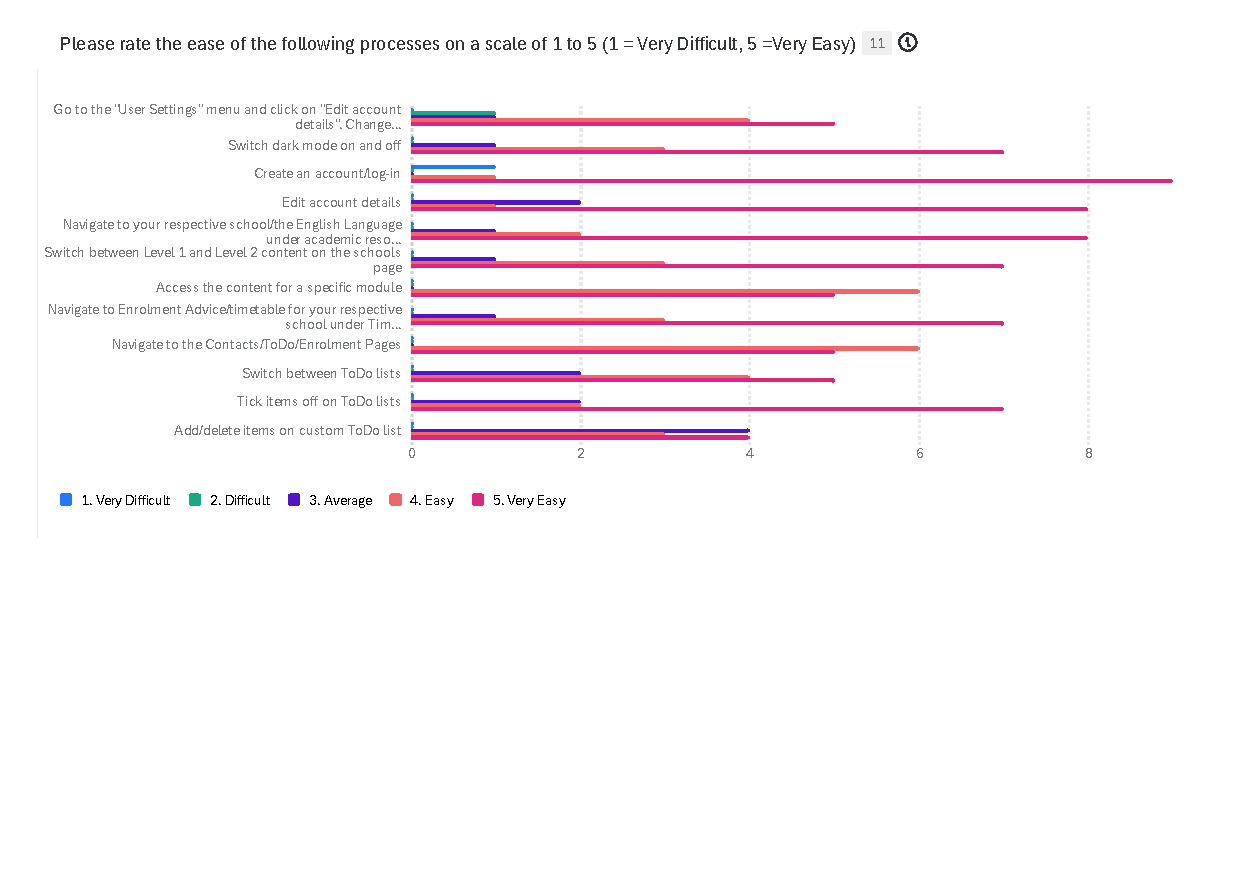
\includegraphics[width=\linewidth]{images/uniStudentsDifficulty.pdf}    
        \caption{Difficulty rating of each task from university student evaluation.}
        \label{fig:uniDifficulty} 
    \end{subfigure}
    \centering
    \begin{subfigure}[b]{\textwidth}
        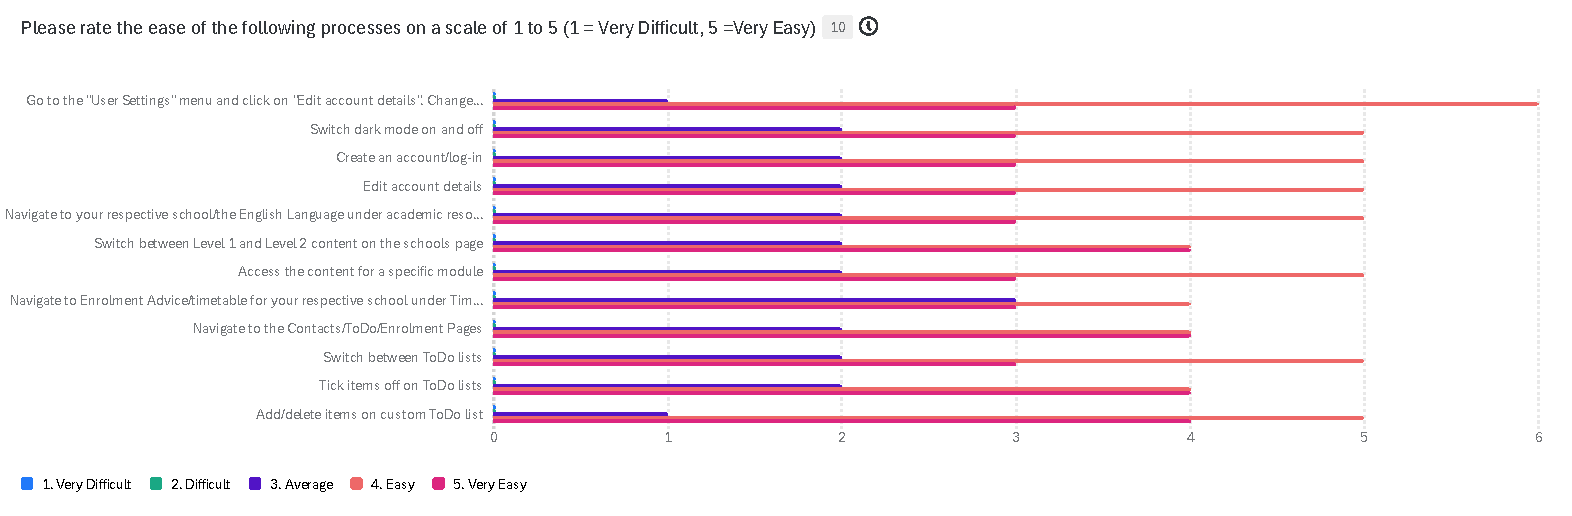
\includegraphics[width=\linewidth]{images/highschoolStudentsDifficulty.pdf}    
        \caption{Difficulty rating of each task from high school student evaluation.}
        \label{fig:highschoolDifficulty} 
    \end{subfigure}
    ~ %add desired spacing between images,  e. g. ~,  \quad,  \qquad,  \hfill etc. 
    %(or a blank line to force the subfigure onto a new line)    
    \caption{Difficulty ratings of each task from each evaluation. \subref{fig:uniDifficulty} shows the ratings from the university student evaluation,  whereas \subref{fig:highschoolDifficulty} shows the ratings from the high school student evaluation.
    }\label{fig:difficulty}
\end{figure}

All of the participants mentioned above were able to complete all tasks. For the tasks "Go to the "User Settings" menu and click on "Edit account details". Change your password and follow the instruction on the screen" and "Create an account/log-in",  one university student participant rated them "difficult" and "very difficult" respectively. One participant stated that it was "very difficult to log in as a new user" when asked what they disliked most about the application. As for the high school participants, 100\% found all the tasks to be "average" to "very easy" to carry out. There was no noticeable difference in difficulty rating between those planning on studying chemistry or physics or both at university, and those planning on studying something different.

Figure \ref{fig:experience} shows the results of the user experience questions. As can be seen the majority of participants "agree" or "strongly agree" with the statements,  with a some of participants rating "neutral" for some. The outcome from this is that the application is very well put together,  and achieves getting across the relative information efficiently with little loading while being easily navigable for users. The comments and responses provided by the university student evaluation reinforce this as they reflect the importance of an application such as this. While those who completed the high school evaluation might not be an offer holder, they will perhaps see more of a benefit to the application should they receive an offer and take a proper look into it.

\begin{figure}[ht]
    \centering
    \begin{subfigure}[b]{\textwidth}
        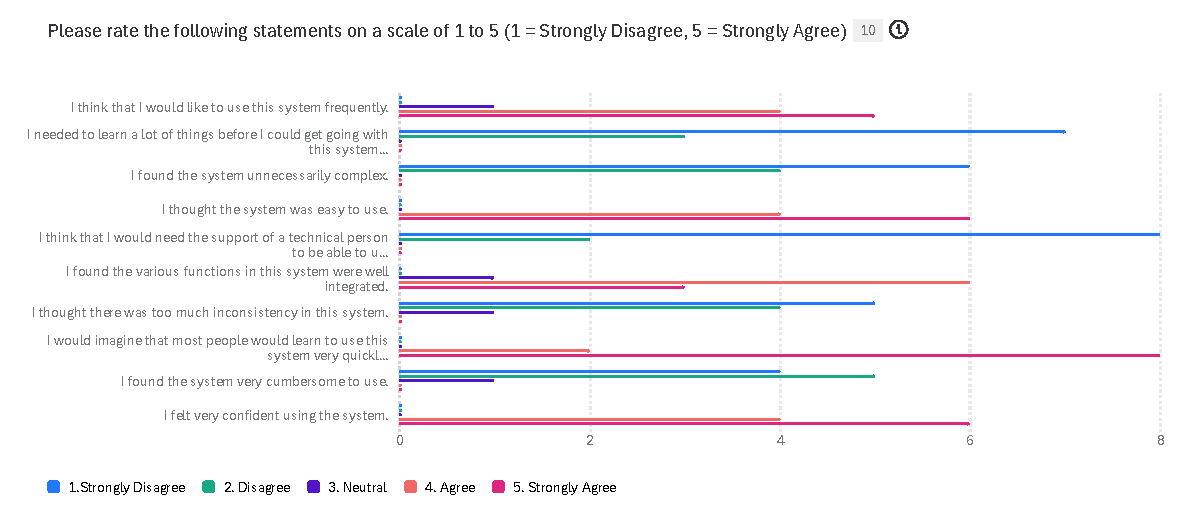
\includegraphics[width=\linewidth]{images/uniStudentsExperience.pdf}    
        \caption{User experience rating from university student evaluation.}
        \label{fig:uniExperience} 
    \end{subfigure}
    \centering
    \begin{subfigure}[b]{\textwidth}
        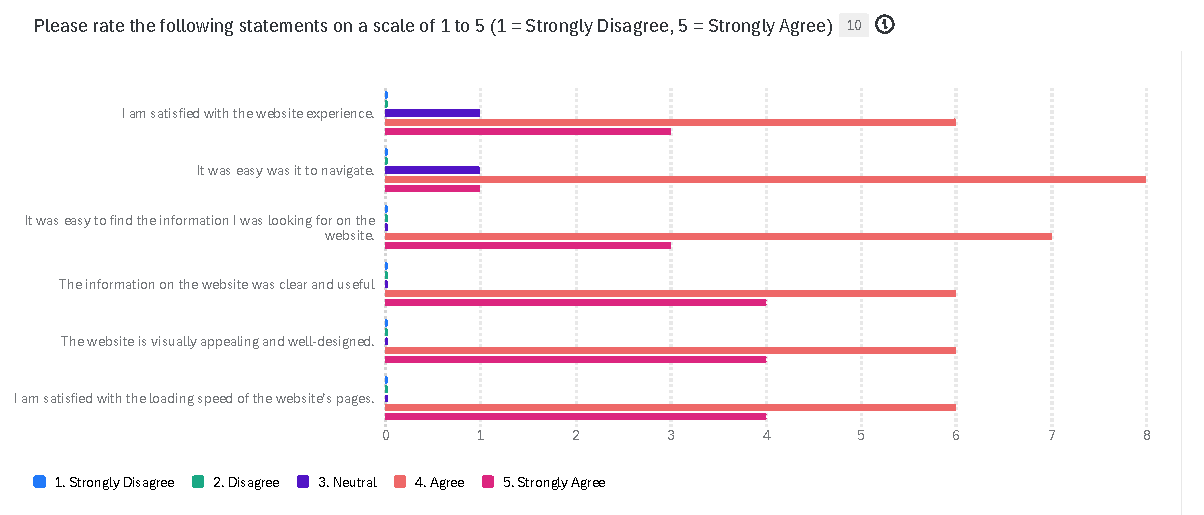
\includegraphics[width=\linewidth]{images/highschoolStudentsExperience.pdf}    
        \caption{User experience rating from high school student evaluation.}
        \label{fig:highschoolExperience} 
    \end{subfigure}
    ~ %add desired spacing between images,  e. g. ~,  \quad,  \qquad,  \hfill etc. 
    %(or a blank line to force the subfigure onto a new line)    
    \caption{User experience ratings from each evaluation. \subref{fig:uniExperience} shows the ratings from the university student evaluation,  whereas \subref{fig:highschoolExperience} shows the ratings from the high school student evaluation.
    }\label{fig:experience}
\end{figure}

\subsubsection{Improvements}
Most comments made when participants were asked what they disliked most about the application said nothing and praised the application. Suggestions provided by students here were only for small additional features and fixed. One comment touched on the UI of the "What kind of chemist are you?" quiz on the homepage. As this quiz is an external resource provided by the School of Chemistry no fixes can be made from this project,  however,  the feedback has been passed on to the representatives from the school. Another student said they disliked that the application was only for Level 1 and 2 students.

\subsubsection{Summary}
Overall the results suggest that users find the application easy to navigate and use. Users are satisfied with the experience using the application,  with comments from participants being overall positive. Comments particularly praised the applications for being easy to navigate and the information provided for being useful.

Features were suggested to improve the application in future.

\subsection{Limitations} \label{evalLims}
The unobserved nature of this evaluation meant that it was difficult to ensure that all participants completed the evaluation in full. As a result of this fewer results were gathered than could have been as seen by the responses to the completed evaluation ratio. Additional information such as the device used was also impossible to gather as a result of this. A question was added to the user demographic questions after the initial deployment of the evaluation,  but by that point,  there were already some respondents making it invalid going forward.

\section{System Usability Scale}
Following answering the questions related to the task and the application experience,  participants were asked to fill out a System Usability Scale (SUS) questionnaire. The SUS questionnaire is a widely used method of measuring system usability as perceived by the user \citep{lewis2018system}. The SUS questionnaire was chosen for a variety of reasons. The first was that the method has been used for a long time to measure usability and is recognised widely to be accurate and successful. Secondly,  participants do not need to invest a large amount of time to complete the questionnaire. Finally,  the questionnaire is easy and cost-effective to run.

\subsection{What is the SUS Questionnaire?}
Participants are asked to rate the following 10 statements from 1 to 5,  with 1 being strongly disagree and 5 being strongly agree,  stating whether they agree with each statement or not \citep{T_2021}:
\begin{itemize}
    \item I think that I would like to use this system frequently
    \item I needed to learn a lot of things before I could get going with this system
    \item I found the system unnecessarily complex
    \item I thought the system was easy to use
    \item I think that I would need the support of a technical person to be able to use this system
    \item I found the various functions in this system were well integrated
    \item I thought there was too much inconsistency in this system
    \item I would imagine that most people would learn to use this system very quickly
    \item I found the system very cumbersome to use
    \item I felt very confident using the system
\end{itemize}

The full SUS questionnaire can be viewed as part of the evaluation surveys in Appendix \ref{app:evalSurvey}.

\subsection{Results}
A SUS score was calculated for each participant's response. This score was calculated by taking the sum of values under the following conditions and multiplying it by 2.5 \citep{T_2021}:
\begin{itemize}
    \item \textbf{Odd Questions:} Answer - 1
    \item \textbf{Even Questions:} 5 - answer
\end{itemize}
Following this the score can fall under one of the following categories:
\begin{itemize}
    \item \textbf{Awful:} $<$51
    \item \textbf{Poor:} 51-68
    \item \textbf{Okay:} 68
    \item \textbf{Good:} 68-80.3
    \item \textbf{Excellent:} $>$80.3
\end{itemize}
For the current university students,  an average score of \textbf{88.5} was calculated,  and therefore falls into the "excellent" category. For the students currently in high school,  the average score was \textbf{70.5},  falling under the "good" category. Therefore according to the SUS method,  it can be concluded that overall participants found the usability of the system to be a positive experience. A breakdown of the occurrences in each category and the distribution can be seen in Figures \ref{fig:susDistribution} and \ref{fig:susOccurences}

The lower usability score from the high school students could be down to the overall style and layout of the website. Since it was loosely based on the University of Glasgow Moodle,  those who are currently university students would be more familiar with a system that similarly operates both physically and functionality.

\begin{figure}[ht]
    \centering
    \includegraphics[width=0.7\linewidth]{images/susDistribution.pdf}    

    \caption{SUS scores distribution falling under the categories "awful" to "excellent" as based on SUS score interpretation table by \cite{T_2021}
    }

    % use the notation fig:name to cross reference a figure
    \label{fig:susDistribution} 
\end{figure}

\begin{figure}[ht]
    \centering
    \includegraphics[width=0.7\linewidth]{images/susOccurences.pdf}    

    \caption{Number of participants SUS scores falling under the categories "awful" to "excellent" as based on SUS score interpretation table by \cite{T_2021}
    }

    % use the notation fig:name to cross reference a figure
    \label{fig:susOccurences} 
\end{figure}

\subsection{Limitations}
20\% of participants gave the application a SUS score falling under "awful" and "poor",  as can be seen in Figure \ref{fig:susDistribution}. To help decide what improvements could be made in future work on the application,  it would be useful to collect more feedback from these participants about what areas of the system they encountered problems with or found difficult to use. Unfortunately,  the anonymity of the SUS questionnaire makes it impossible to schedule follow-up interviews.

\section{Meeting with Transitions Working Group} \label{TWG}
The Transitions Working Group at the University of Glasgow requested the application be presented to them at one of their meetings. During this meeting,  the background of the project was covered before moving onto a live demonstration of the application. From the ten attendees of the meeting,  the feedback provided was positive,  with interest shown for a system like this being made available to all schools and colleges in the University. A comment was made on the computer science transition application as discussed in Chapter \ref{background},  and it was mentioned that this application was implemented with the intention of being able to combine the two applications together in future under the UofG Prepare title.

Following from this meeting the unobserved evaluation was sent out to the attendees of the meeting. Of the four who opened the evaluation,  only one completed it,  providing positive feedback,  and additionally adding positive comments on the "overall light-touch UofG brand feel". The one attendee who completed the evaluation also gave the system a SUS score of \textbf{92.5},  falling under the "excellent" category.

\section{Aims and Requirements Analysis}
This section looks back at the requirements discussed in Chapters \ref{Intro} and \ref{Requierments},  and reflects on whether they have been met or not.

\subsection{Aims}
Comments from the end of the evaluations were taken into account to check if the aims of the application as discussed in Chapter \ref{Intro} had been achieved.

\subsubsection{Prepare students for life at the University of Glasgow.}
One participant commented that "the information present was something I would have found useful as an incoming student",  with another stating "I would have liked to have had something like this before I started first year so that I would have felt more prepared to start the year". The main area of the application is that of Academic Resources,  which contains specialised information about all the modules covered in Level 1 and 2 chemistry and physics. Many participants praised the inclusion of these,  with one participant in particular stating that they "would have been less stressed as I would have had a better understanding of what the structure of the course was going to look like" before starting their studies. The application delivers essential information and contacts for incoming students through its to-do list and contacts section. Walking incoming students through what they need to-do before they come to university,  and guiding them to the right areas for additional assistance. The application has a simplistic design where it is "Easy to find stuff" as one participant commented. Furthermore,  the application directs users to external sources where they can find out more information about extracurricualrs available to them to enhance their university experience.

\subsubsection{Easily Accessible Anywhere,  Anytime.}
The application does not require an account to be accessed making it available to everyone. The mobile-responsiveness of the application means it can be accessed on any device as long as a web browser is downloaded and the user has internet connection. As a result,  the application is anywhere and anytime provided the user has internet access.

\subsubsection{Editable and Expandable.}
The application can be edited by users in the personal to-do list area. For edits to the applications main content then changes to the code base would have to be made. This is due to the information being coded into the application statically. This could have been avoided by hosting the applications content in the database and reading it in. The application is expandable and has been built and designed in a way which all schools and colleges at the University of Glasgow could have their own area of the application dedicated to their specific content.

\subsection{Functional Requirements}
Table \ref{tab:functional} shows the functional requirements discussed at the end of Chapter \ref{requirements},  and whether they have been satisfied. Only the requirements that fell under \textbf{Must Have} are included. The full table can be viewed in Appendix \ref{app:reqMet}. In short,  all \textbf{Must Have} requirements have been satisfied.

\begin{table}[ht]
    \caption{Table showing the functional requirements of the application,  the MoSCoW category they fall under,  whether they are satisfied,  and reasoning for their status. }\label{tab:functional}
    %\tt 
    \rowcolors{2}{}{gray!3}
    \begin{tabular}{ m{3cm}  m{2cm}  m{1.5cm}  m{17em} }
    %\toprule
    \hline
    \textbf{Requirement}    & \textbf{Category}                & \textbf{Satisfied}      & \textbf{Reason}                      \\ %\midrule % optional rule for header
    \hline
    
    Overview of Modules  &  Must Have              & Yes                 & The application provides a breakdown of each module covered in both Levels 1 \& 2 chemistry and physics as an overview and the aims. \\

    External English Language Resources & Must Have & Yes & The application contains a whole page dedicated to redirecting users to external language learning resources. \\

    Example Timetables & Must Have & Yes & The application provides an example of the chemistry and physics timetable fro both semester for Levels 1 \& 2. \\

    Pre-University To-Do List & Must Have & Yes & The application provides to-do lists telling users about tasks and items they should have completed before starting and that they should do in their first week. \\
    
    Links to Disability Service & Must Have & Yes & The contacts section of the application redirects users to the universities disabilities service page. \\
    
    Essential Contacts & Must Have & Yes & The application contains a section holding the key contacts that both schools wished to provide to incoming students.

    % \bottomrule
    \end{tabular}
\end{table}

\subsection{Non-Functional Requirements}
Table \ref{tab:non-functional} shows all the non-functional requirements discussed at the end of Chapter \ref{requirements},  and whether they have been satisfied. The requirements that fell under \textbf{Won't Have} are not included. In short,  all have been at least partially satisfied.

\begin{table}[ht]
    \caption{Table showing the non-functional requirements of the application,  the MoSCoW category they fall under,  whether they are satisfied,  and reasoning for their status. }\label{tab:non-functional}
    %\tt 
    \rowcolors{2}{}{gray!3}
    \begin{tabular}{ m{3cm}  m{2cm}  m{1.5cm}  m{17em} }
    %\toprule
    \hline
    \textbf{Requirement}    & \textbf{Category}                & \textbf{Satisfied}      & \textbf{Reason}                      \\ %\midrule % optional rule for header
    \hline
    
    Accessible & Must Have & Yes & The application can be used without having to create an account. \\

    Mobile Responsive & Must Have & Yes & The application responds to being opened on a mobile device. \\

    Easy to Use& Must Have & Yes & The application is easy to navigate and use. \\

    Fast Load Times & Should Have & Yes & The application loads in less than 2 seconds. \\
    
    Handle High Traffic & Should Have & Yes & The system does not buffer or slow down when there is high traffic. \\
    
    Real-time Updates & Should Have & Yes & \textbf{Firebase Realtime database} means that data is updated in real-time. \\

    Editable & Should Have & Partially & The schools can edit content in the application,  however,  they would need to go through the code base.\\

    Expandable & Should Have & Partially & The schools can add content to the application,  however they would need to go through the code base. \\
    
    Dark mode & Could Have & Yes & It was found that user preference helps with the user experience,  so this was included.

    % \bottomrule
    \end{tabular}
\end{table}


\section{Limitations}
It would have been useful to have tested the application with some Glasgow International College students preparing to enter into Level 2. That said however,  the feedback from current University of Glasgow students and staff from both schools,  the transitions working group at the University of Glasgow,  and the students from a greater Glasgow area high school who are preparing to enter university was useful as it provided a perspective from those preparing to go through,  those who have gone through,  and those with experience aiding incoming student with the transition process.

Quantitative data was impossible to collect from this application. Were this to be collected incoming students would have had to have been monitored using the application throughout their whole transition period. That is from before starting university to the end of their first year of studies. This would have provided data on the impact the application had on student progression rates and GPA.

%==================================================================================================================================
\chapter{Conclusion}
\section{Summary}
This project aimed to develop an application to assist students transitioning into higher education chemistry and physics. The transition period is difficult for many students for a variety of reasons. Lots worry about adapting to new surroundings,  while others stress over finances and creating a new routine. Students entering into chemistry and physics stress over their grades and express self-doubt in achieving in the ever-increasing difficulty of the modern curriculum,  however,  through peer learning and easily accessible resources,  they both see improvements in results.

Due to this,  it was important that the application produced by this project took the needs and wants of chemistry and physics students and placed them at the heart of this development. It was important that all the information that they would need for a successful transition period was available in one place,  including contacts and advice about the greater university experience. It was also important that easily accessible summaries of the modules covered in all Level 1 and 2 courses were present to allow students to prepare for their classes before coming to university. Through surveys and discussions with staff and students alike,  it was decided the best way to deliver on these needs was through a web application. While being available on every device should a web browser be installed,  it also meant that the application could be accessed by anyone at any time,  while also familiarising incoming students with similar web applications they will use during their time at university. Building from a previous transition system built by former University of Glasgow student Declan McBride,  the application was taken under the name UofG Prepare: Chemistry and Physics. The application contains summaries of all the modules covered in Levels 1 and 2 chemistry and physics,  highlighting the aims and objectives of each. Additionally,  external language resources are linked to allow incoming students to freshen their English skills preceding starting. It also contains advice on selecting additional modules,  informing users of what is mandatory and what is not. Essential contacts are provided in the application for users who experience issues or need advice in their transition period. Users are provided with to-do lists with tasks they should complete before coming to university and during their induction week. Finally,  links to extracurricular clubs,  societies and student bodies are provided to welcome incoming students to the wider University community. Each feature aims to provide a solution to the many issues and concerns that incoming students from all nationalities and backgrounds have.

The application's evaluation showed that the aims of the application had been satisfied,  as well as all essential functional and non-functional requirements met. Some however had to be reworked or scrapped due to the resources that the schools were able to provide to the project. To fully evaluate the success of the application,  more time would have been required to observe incoming student use of it throughout the transition period. The main issues users had were with logging in and creating an account as a new user,  as well as the UI for an external quiz provided by the School of Chemistry.

\section{Future Work}
Should more time have been allowed for the project the following improvements could have been made.

\subsection{Further Testing}
As mentioned in Section \ref{testing},  \textbf{Cypress.io} was looked into for automated testing. Given more time this package would have been looked into even further and automated test scripts would be written to ensure that every component in the code base was tested.

\subsection{Timetable/To-Do List Mobile Scaling}
The scroll area feature for the timetables and the to-do lists did not work as well as envisioned on mobile view. Time should be taken to investigate ways to make the container components respond to screen resolution or perhaps a zoom-in/out feature.

\subsection{More Content and Abandoned Features}
Given more time the quiz feature should be re-investigated with the representatives from both schools,  with a new, original question bank created for the quizzes. This would allow the feature to be implemented without the issues expressed by both schools originally. If more time were allocated then more recommended and additional materials could be added under the sections in the module pages.

\subsection{University Integration}
The University has its own servers for hosting its systems. To allow the application to be expanded upon and commercialised under the UofG Prepare tag in future,  time should be allocated to integrate the system on the University's servers. It should be noted that the application will be signed off to the University of Glasgow Software Service following the conclusion of the project,  where maintenance and updates will be conducted. Should either school wish to make changes or add content then they should go through the software service.

\section{Final Reflections}
This project has been a fascinating journey exploring educational theory around transition,  as well as the software development process. My knowledge of \textbf{Figma} for prototype and wireframe design has increased as I discovered the extensive library of packages and custom functionalities that can be imported into projects.

I have applied a mixture of software engineering practices I have learned both at university and in industry and have been able to see the importance of using them properly and effectively. Having worked on a pre-existing \textbf{Next.js} application before,  it was challenging building the system from scratch,  but has developed my expertise in these types of systems which will only improve my performance at my current industrial placement. \textbf{Firebase} was learned from the ground up and was interesting and presented challenges along the way. Being able to look further into third-party libraries which I had previously used like \textbf{Mantine} and React-Icons was extremely enjoyable and a staple to creating the UI I had envisioned in the wireframe design.

The evaluation process was by far the biggest and most interesting learning experience. While touched upon in classes,  I never realised the importance of a strong evaluation until this project. Gathering responses,  demonstrating to several groups,  and analysing the results proved challenging but has paved the way to make me a stronger computer scientist going forward. 

Throughout the project,  the importance of time management has been shown to me. I found a struggle to challenge project work with my classes and coursework during the first semester,  however,  approaching the project again following the winter exam diet with a fully structured development plan showed efficiency in catching up where I felt I had fallen behind.

%==================================================================================================================================
%
% 
%==================================================================================================================================
%  APPENDICES  

\begin{appendices}

\chapter{Ethics Checklist} \label{app:ethics}
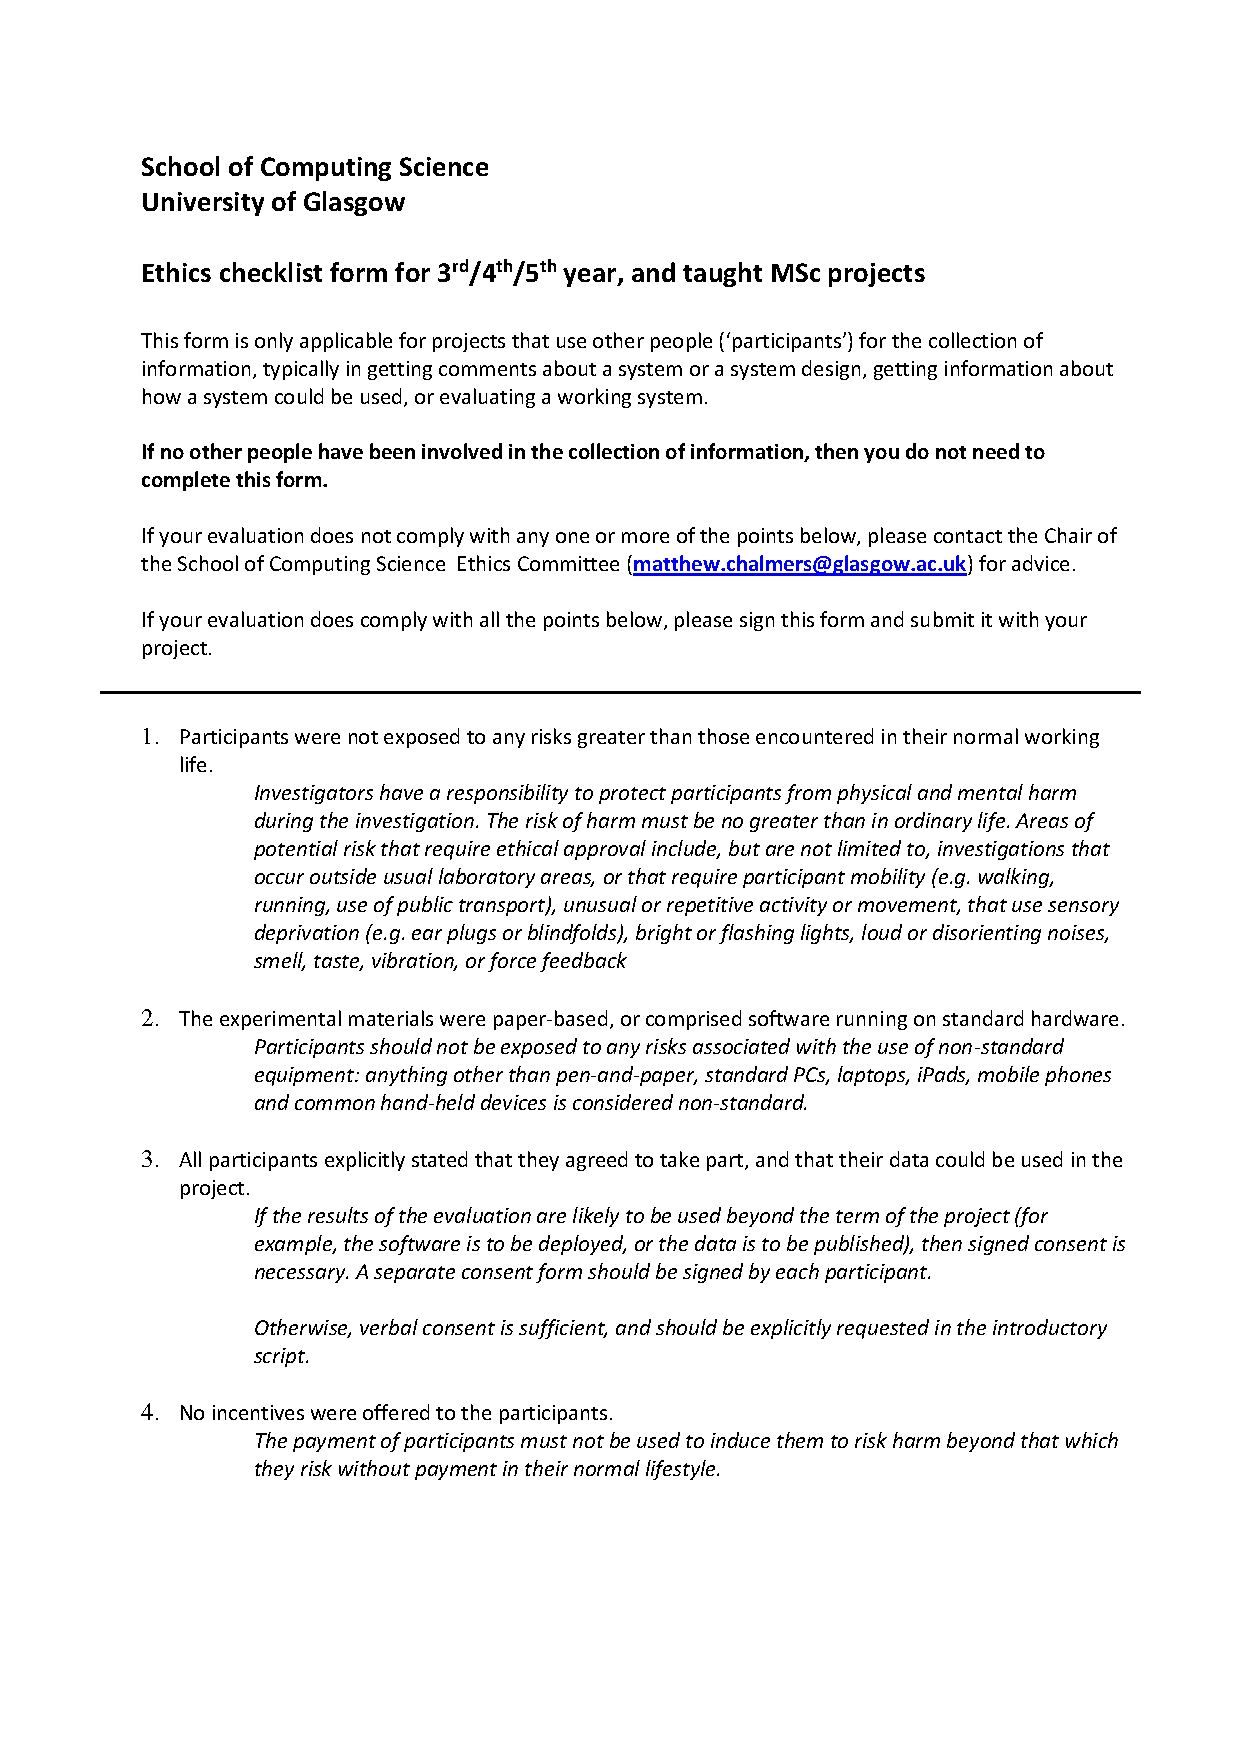
\includepdf[pages=-]{appendix/Ethics_Checklist.pdf}

\chapter{Requirements Gathering} \label{app:requirements}
\section{Initial Ideas} \label{app:initial}
\begin{itemize}
    \item Learn English Section (Useful for International Students [GIC])
    \item Level 1 \& 2 Reading Lists
    \item Level 1 \& 2 Study Guides
    \item Study Tips
    \item Study Tool (Flashcard Maker?,  Quiz at the end of each study guide?)
    \item Essential Contacts (Student Support,  Faster Route Head,  SRC,  Campus Security)
    \item Extracurriculars (Chem Soc, Bio Chem Soc,  Science Soc,  WiSTEM,  Unions,  GUSA,  SRC)
    \item GPA Calculator
\end{itemize}
\section{Requirements Surveys}
\subsection{Chemistry Requirements Survey} \label{app:cehmReqSurvey}
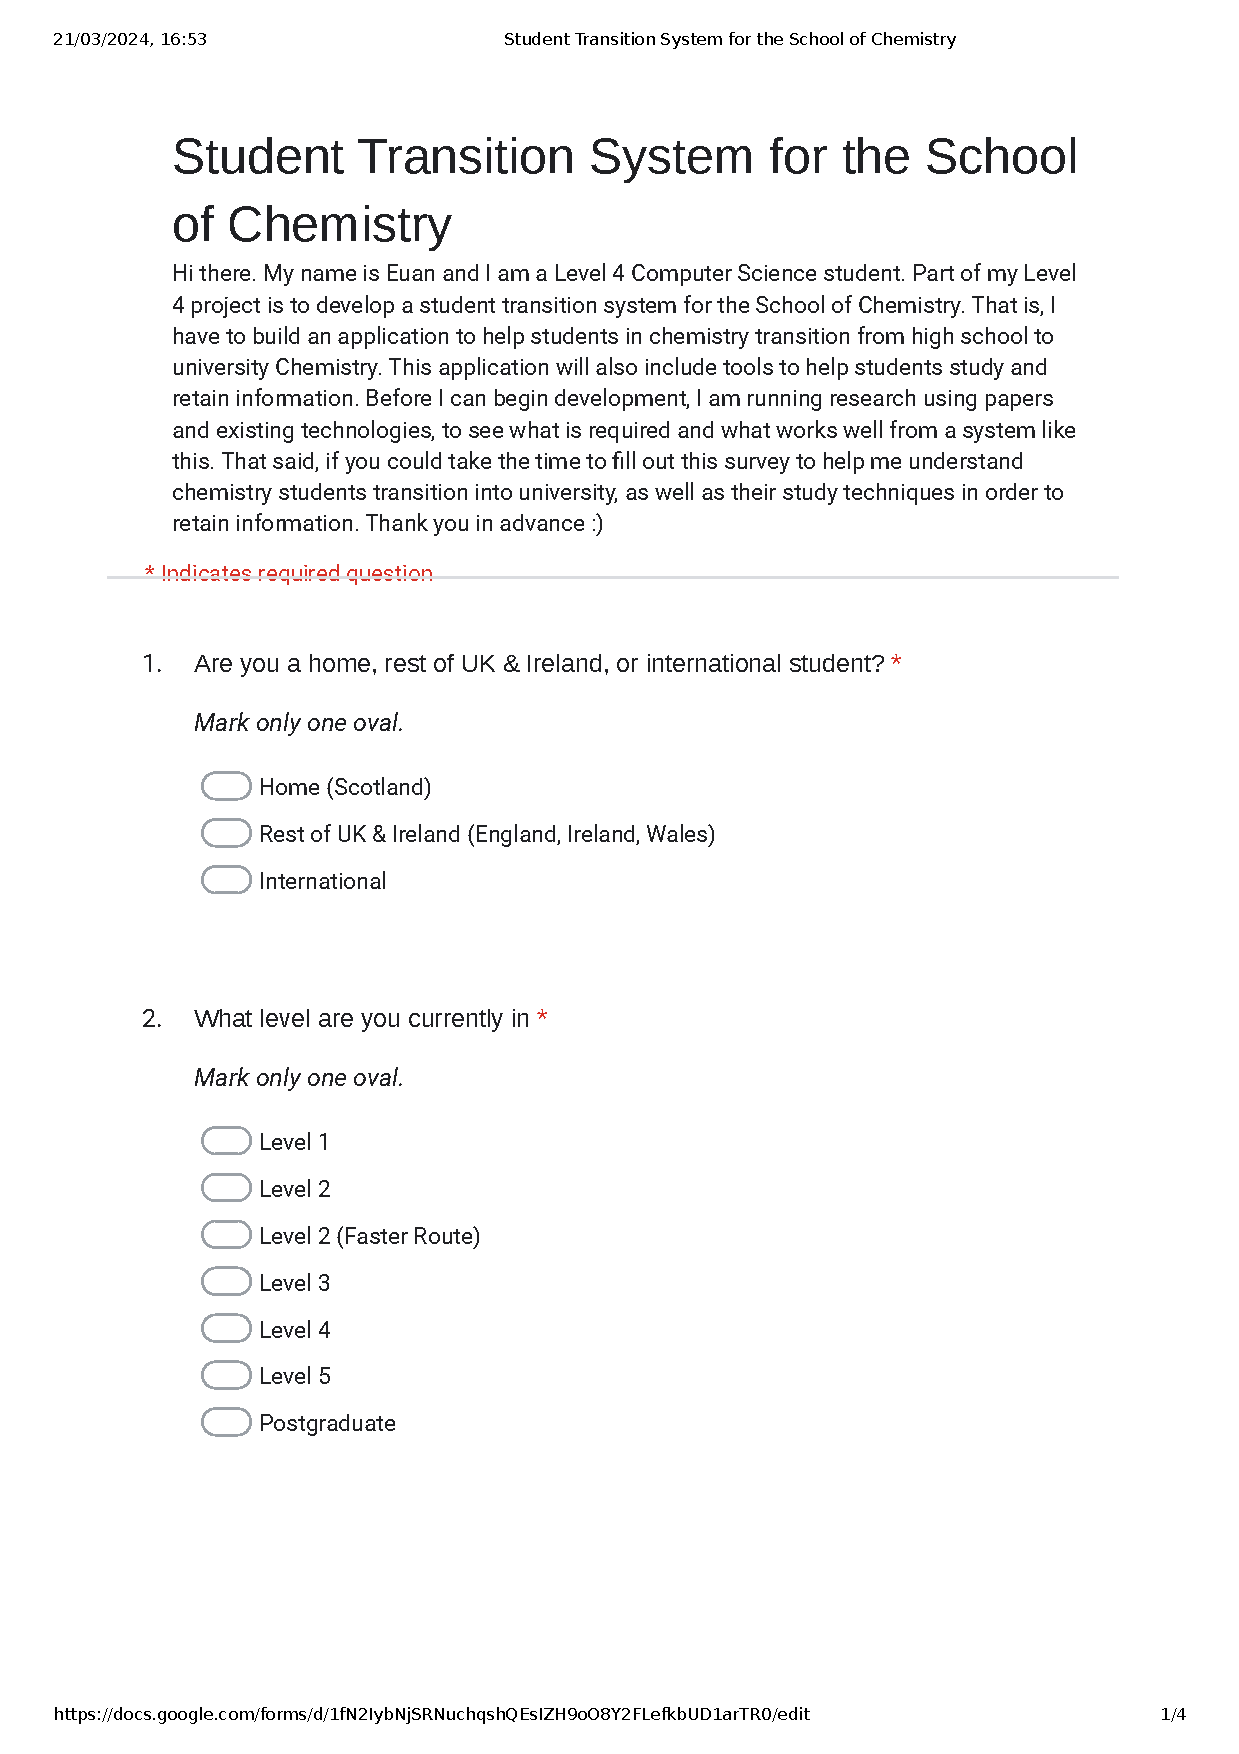
\includepdf[pages=-]{appendix/ChemistryRequirements.pdf}

\subsection{Physics Requirements Survey} \label{app:physReqSurvey}
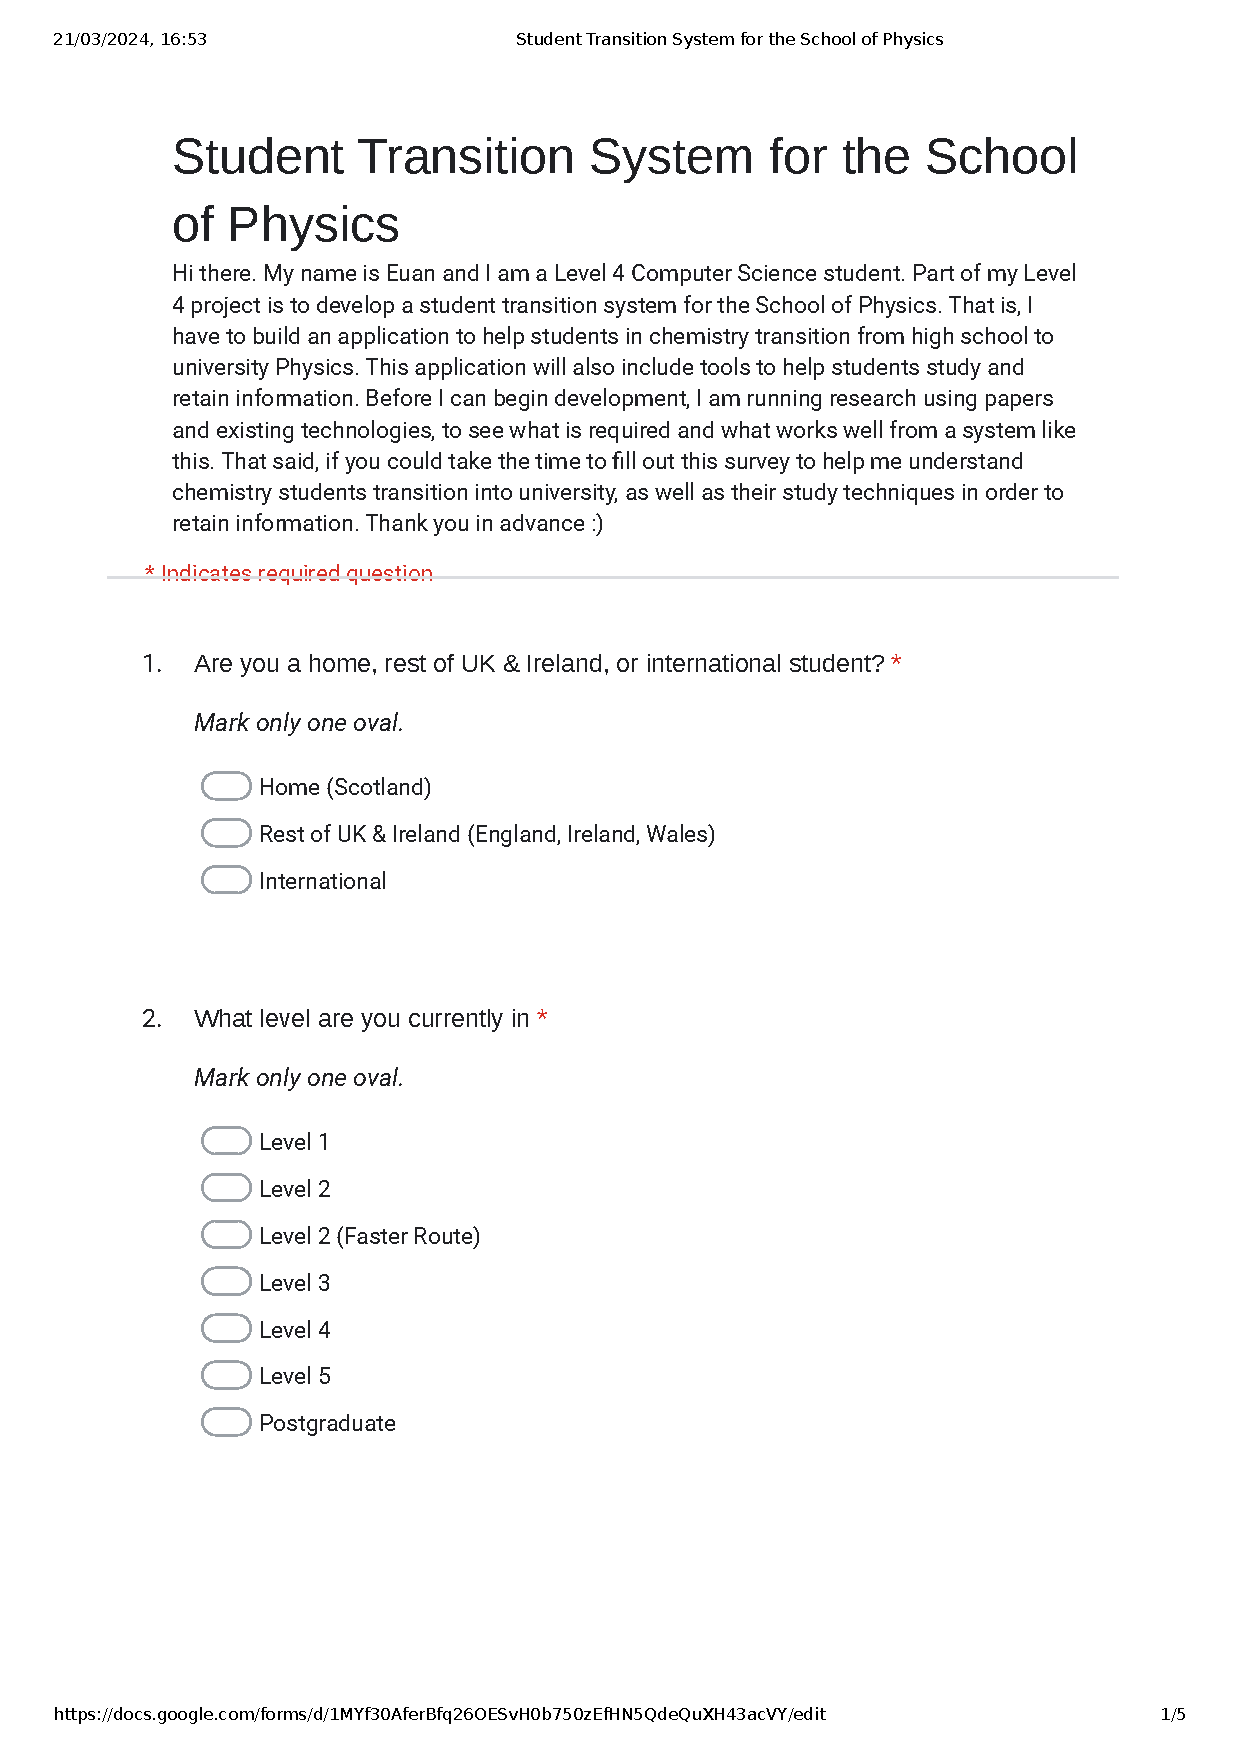
\includepdf[pages=-]{appendix/PhysicsRequirements.pdf}

\section{Survey Results}
\subsection{Chemistry Requirements Survey Results} \label{app:chemReqResults}
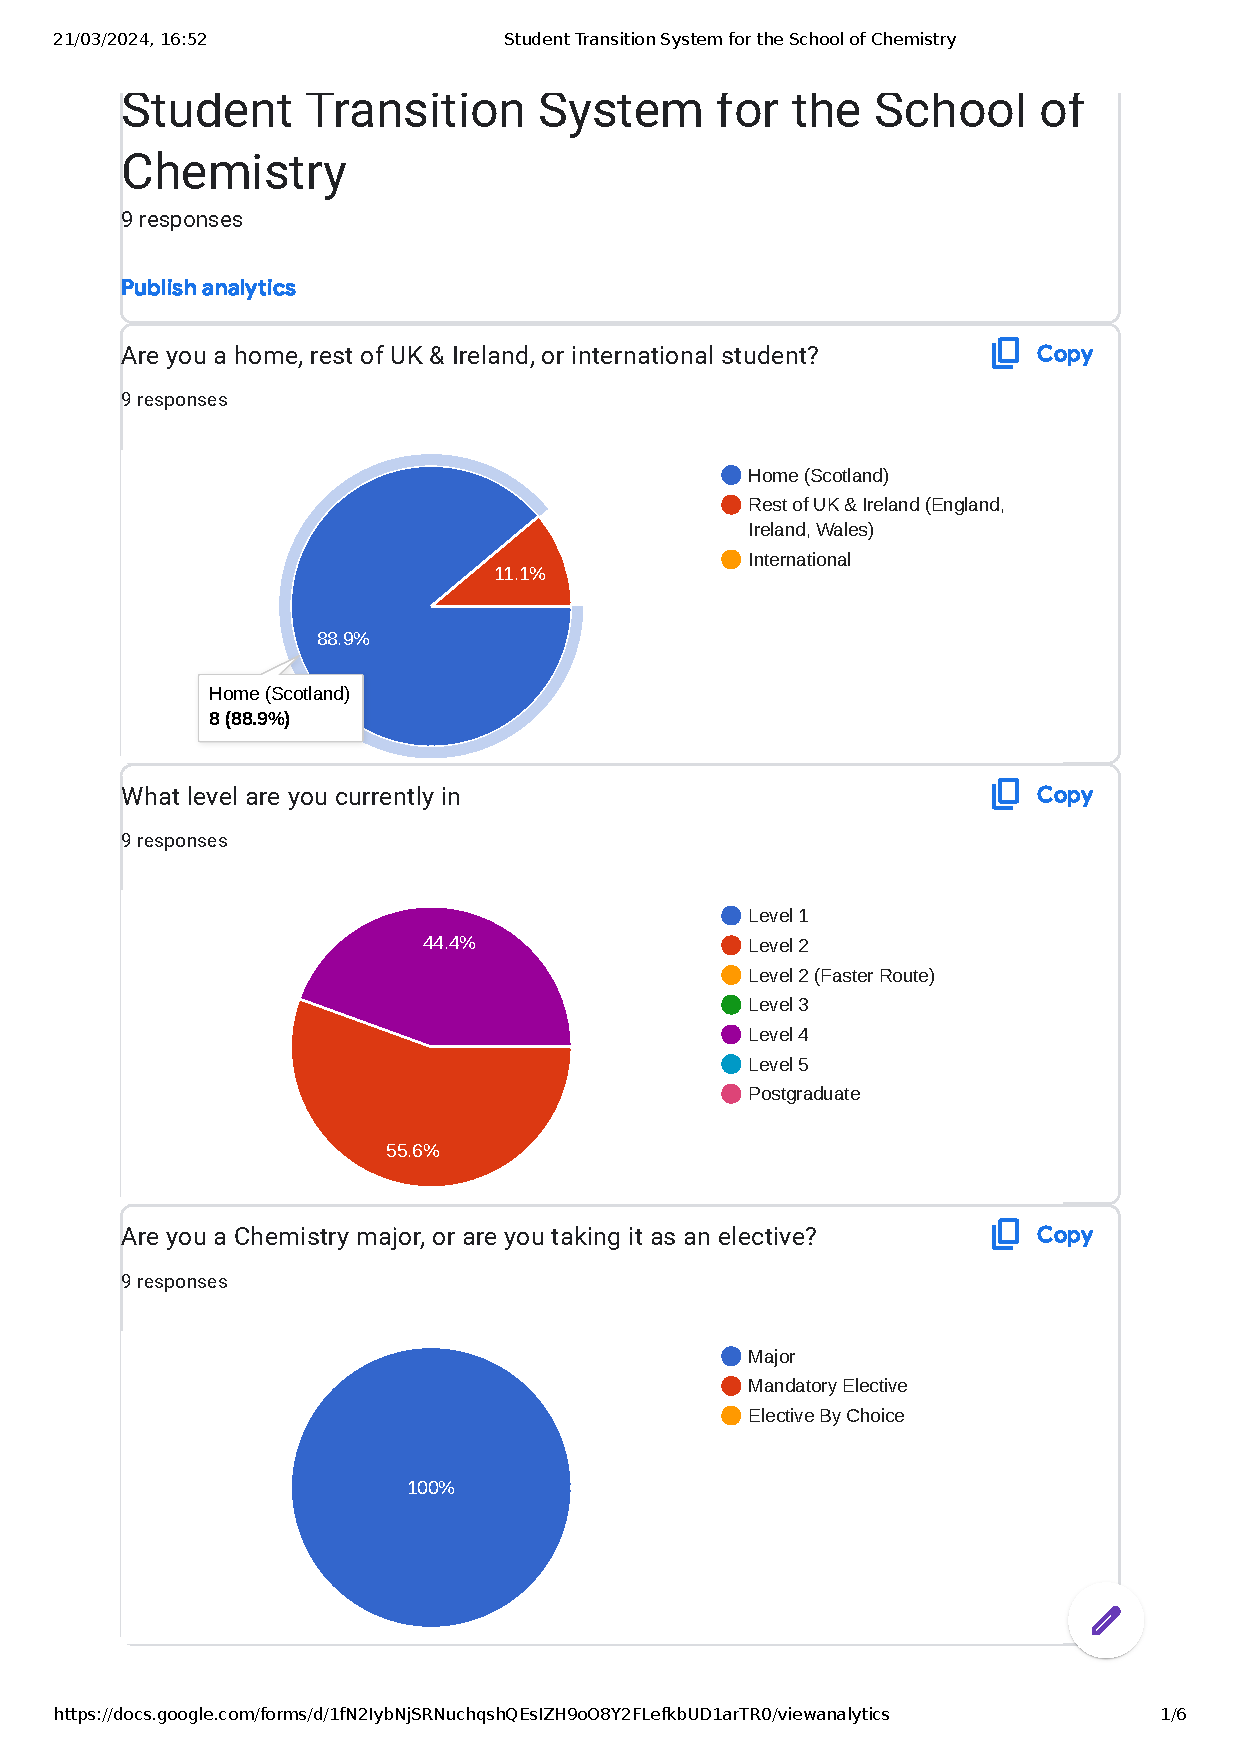
\includepdf[pages=-]{appendix/ChemistryRequirementsResults.pdf}

\subsection{Physics Requirements Survey Results} \label{app:physReqResults}
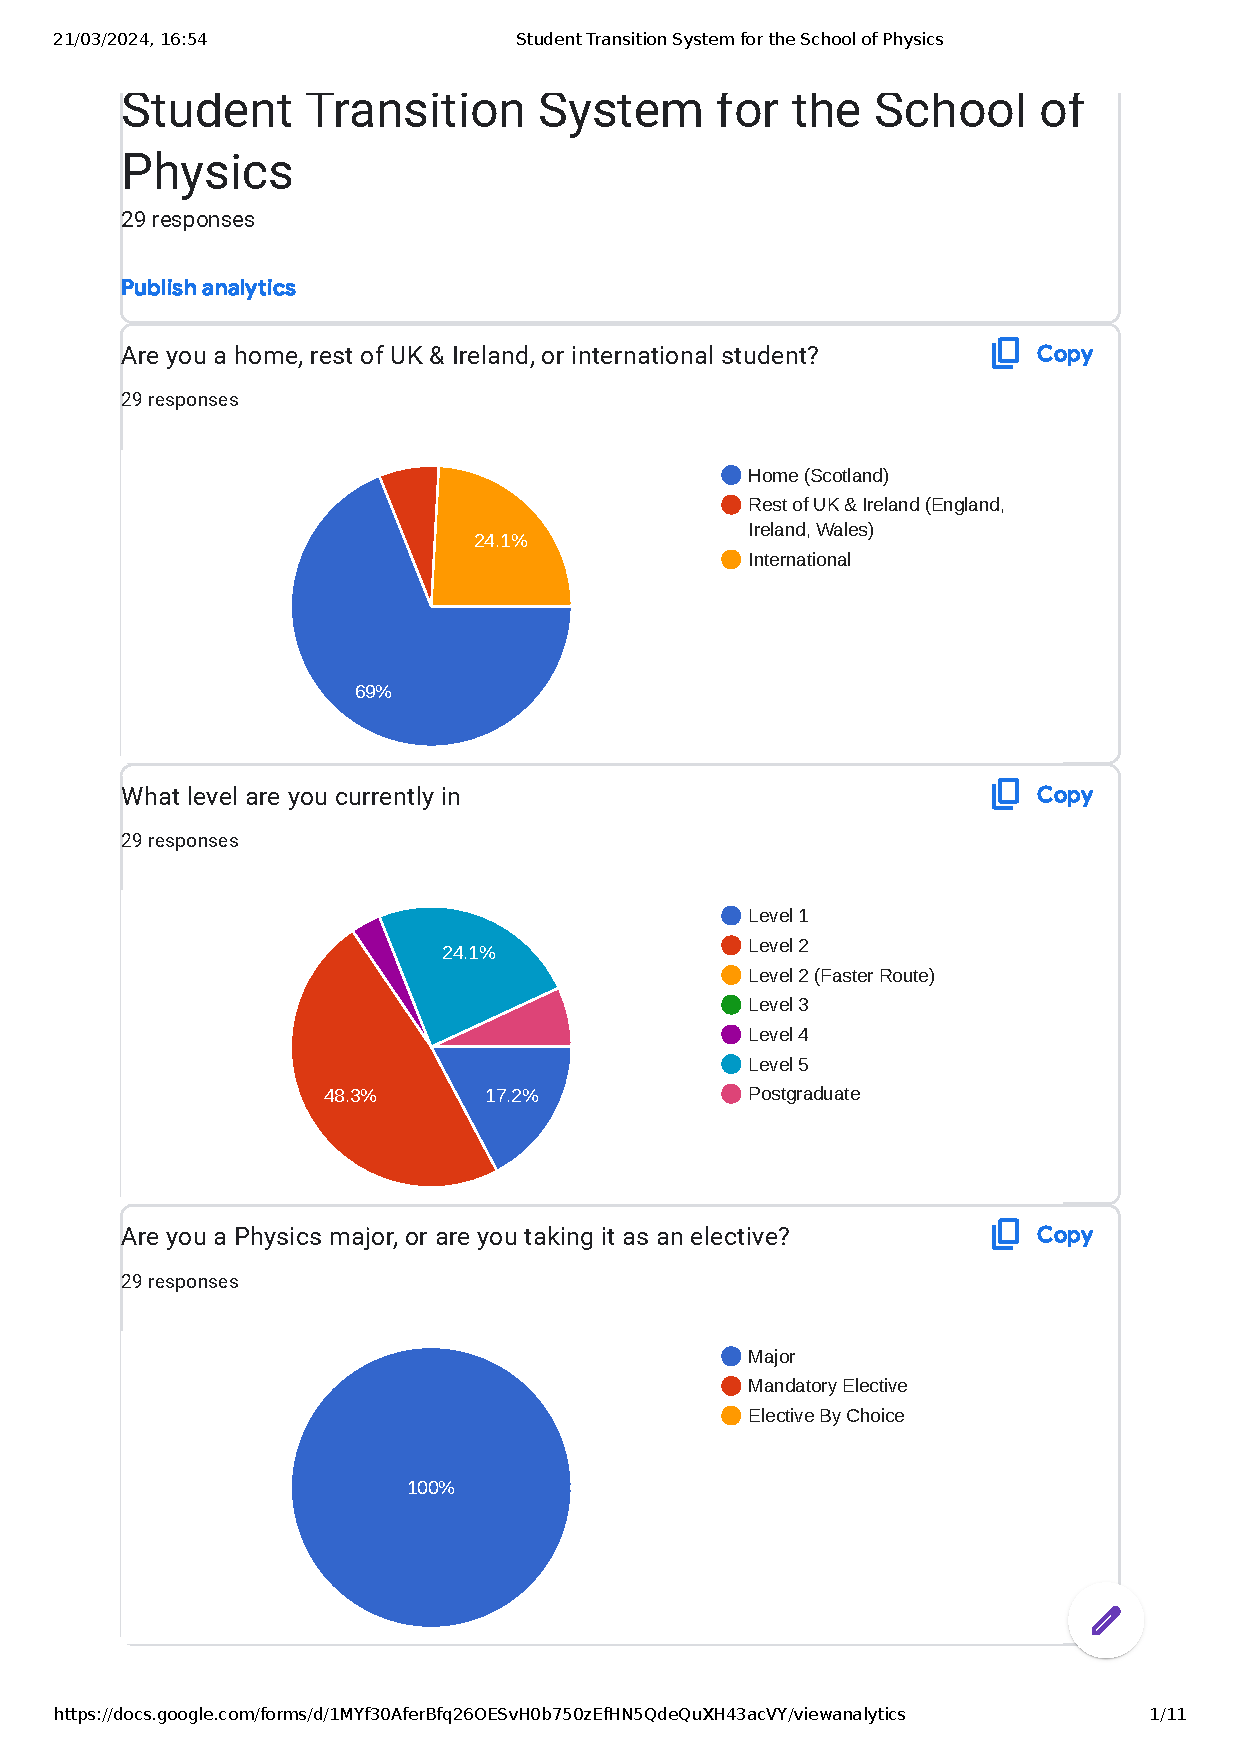
\includepdf[pages=-]{appendix/PhysicsRequirementsResults.pdf}

\chapter{Wireframes and Prototype}
\section{Wireframes} \label{app:wireframes}
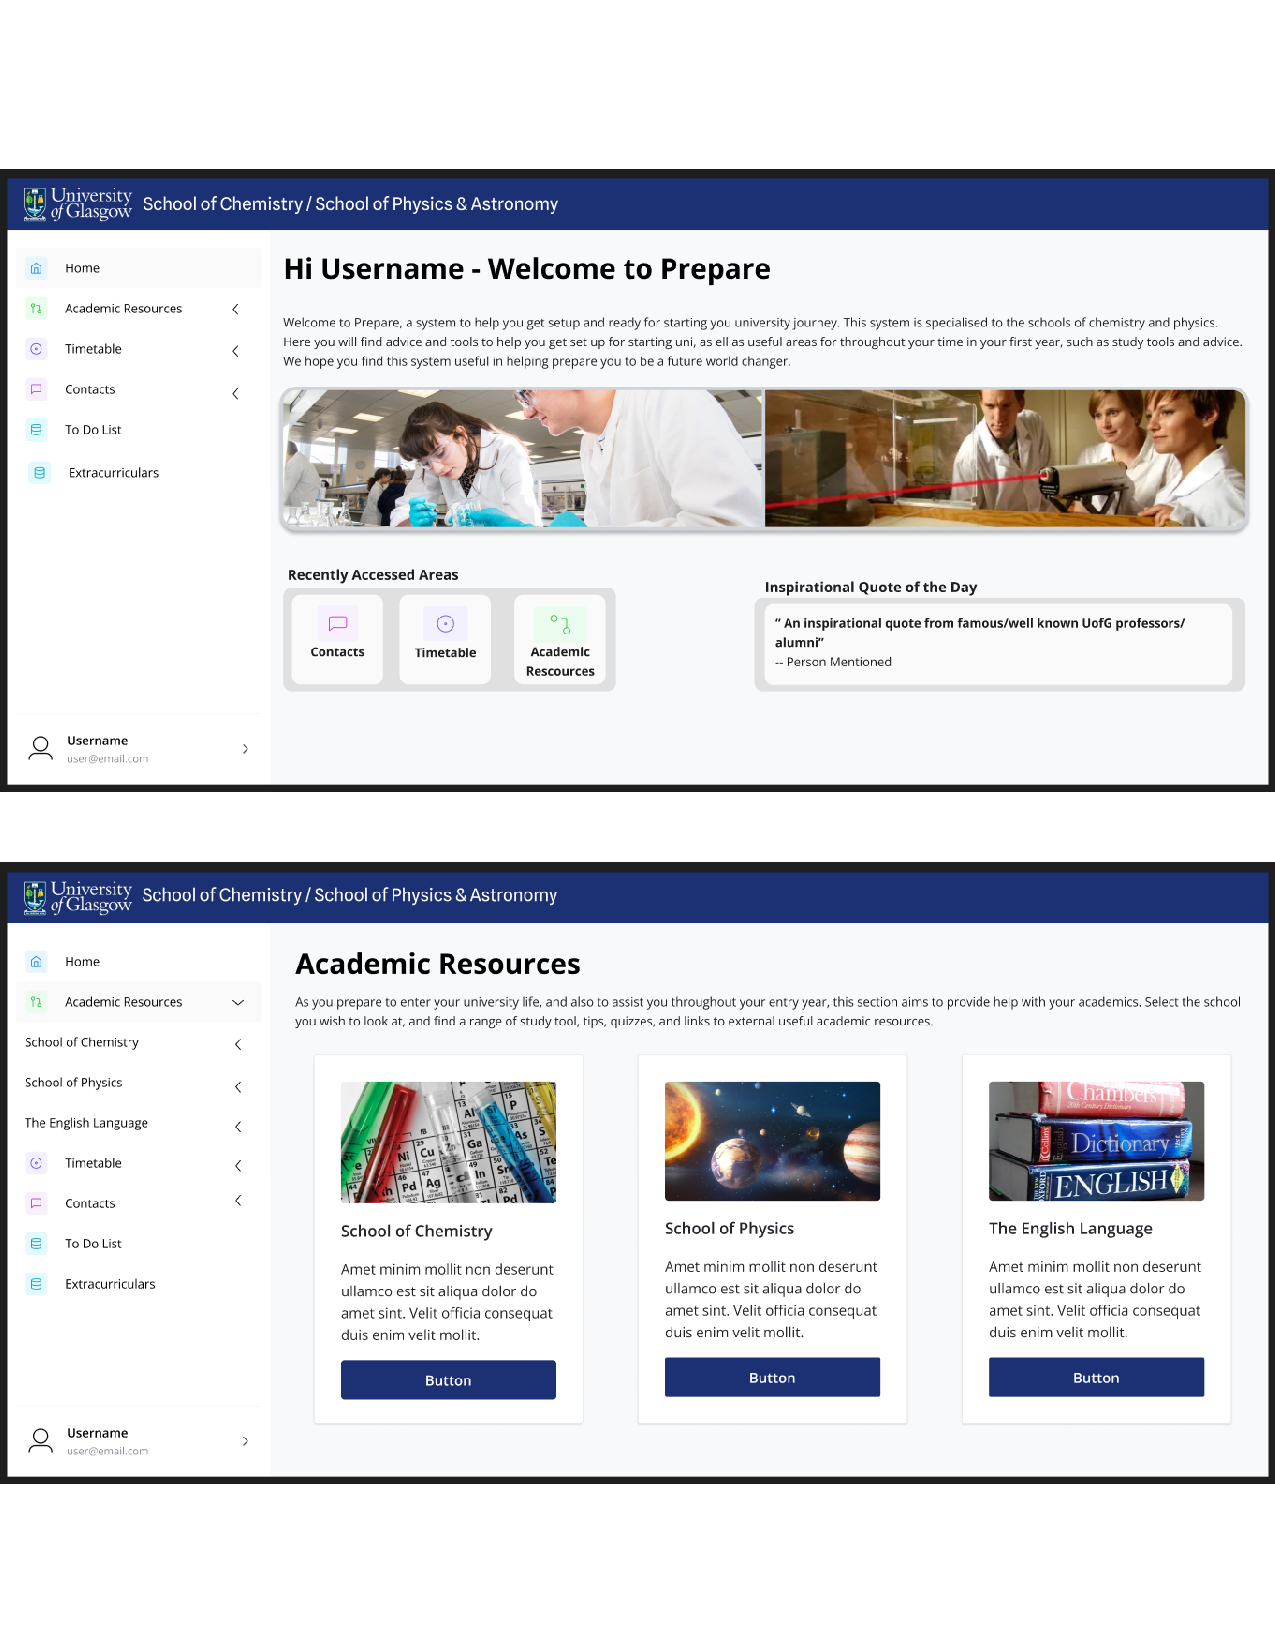
\includepdf[pages=-]{appendix/wireframes.pdf}
Alternatively they can be viewed at the following URL:
\newline
\url{https://www.figma.com/proto/13fIwYm8Y2t1F8r5gq6ppf/Level-4-Project?type=design&node-id=150-4972&t=0m4bBQhped66FFg5-1&scaling=min-zoom&page-id=149%3A3098&starting-point-node-id=150%3A4972&mode=design}

\section{Prototype} \label{app:prototype}
The interactive prototype can be accessed from the following URL:
\newline
\url{https://www.figma.com/proto/13fIwYm8Y2t1F8r5gq6ppf/Level-4-Project?type=design&node-id=150-4972&t=0m4bBQhped66FFg5-1&scaling=min-zoom&page-id=149%3A3098&starting-point-node-id=150%3A4972&mode=design}

\chapter{GitHub Repository}
The GitHub repository for the project can be access at the following URL:
\newline
\url{https://github.com/Eub0/Level4Project/tree/main}

\chapter{Application URL} \label{app:application}
The application can be accessed at the following URL:
\newline
\url{https://uofgprepare.vercel.app/}

\chapter{Video Demonstration} \label{app:video}
A video demonstration of the application was created and can be viewed at the following URL:
\newline
\url{https://youtu.be/dA6WG-f6O0Q}

\chapter{Evaluation} \label{app:eval}
\section{Evaluation Questionnaires} \label{app:evalSurvey}
\subsection{University Student Evaluation} \label{app:evalUni}
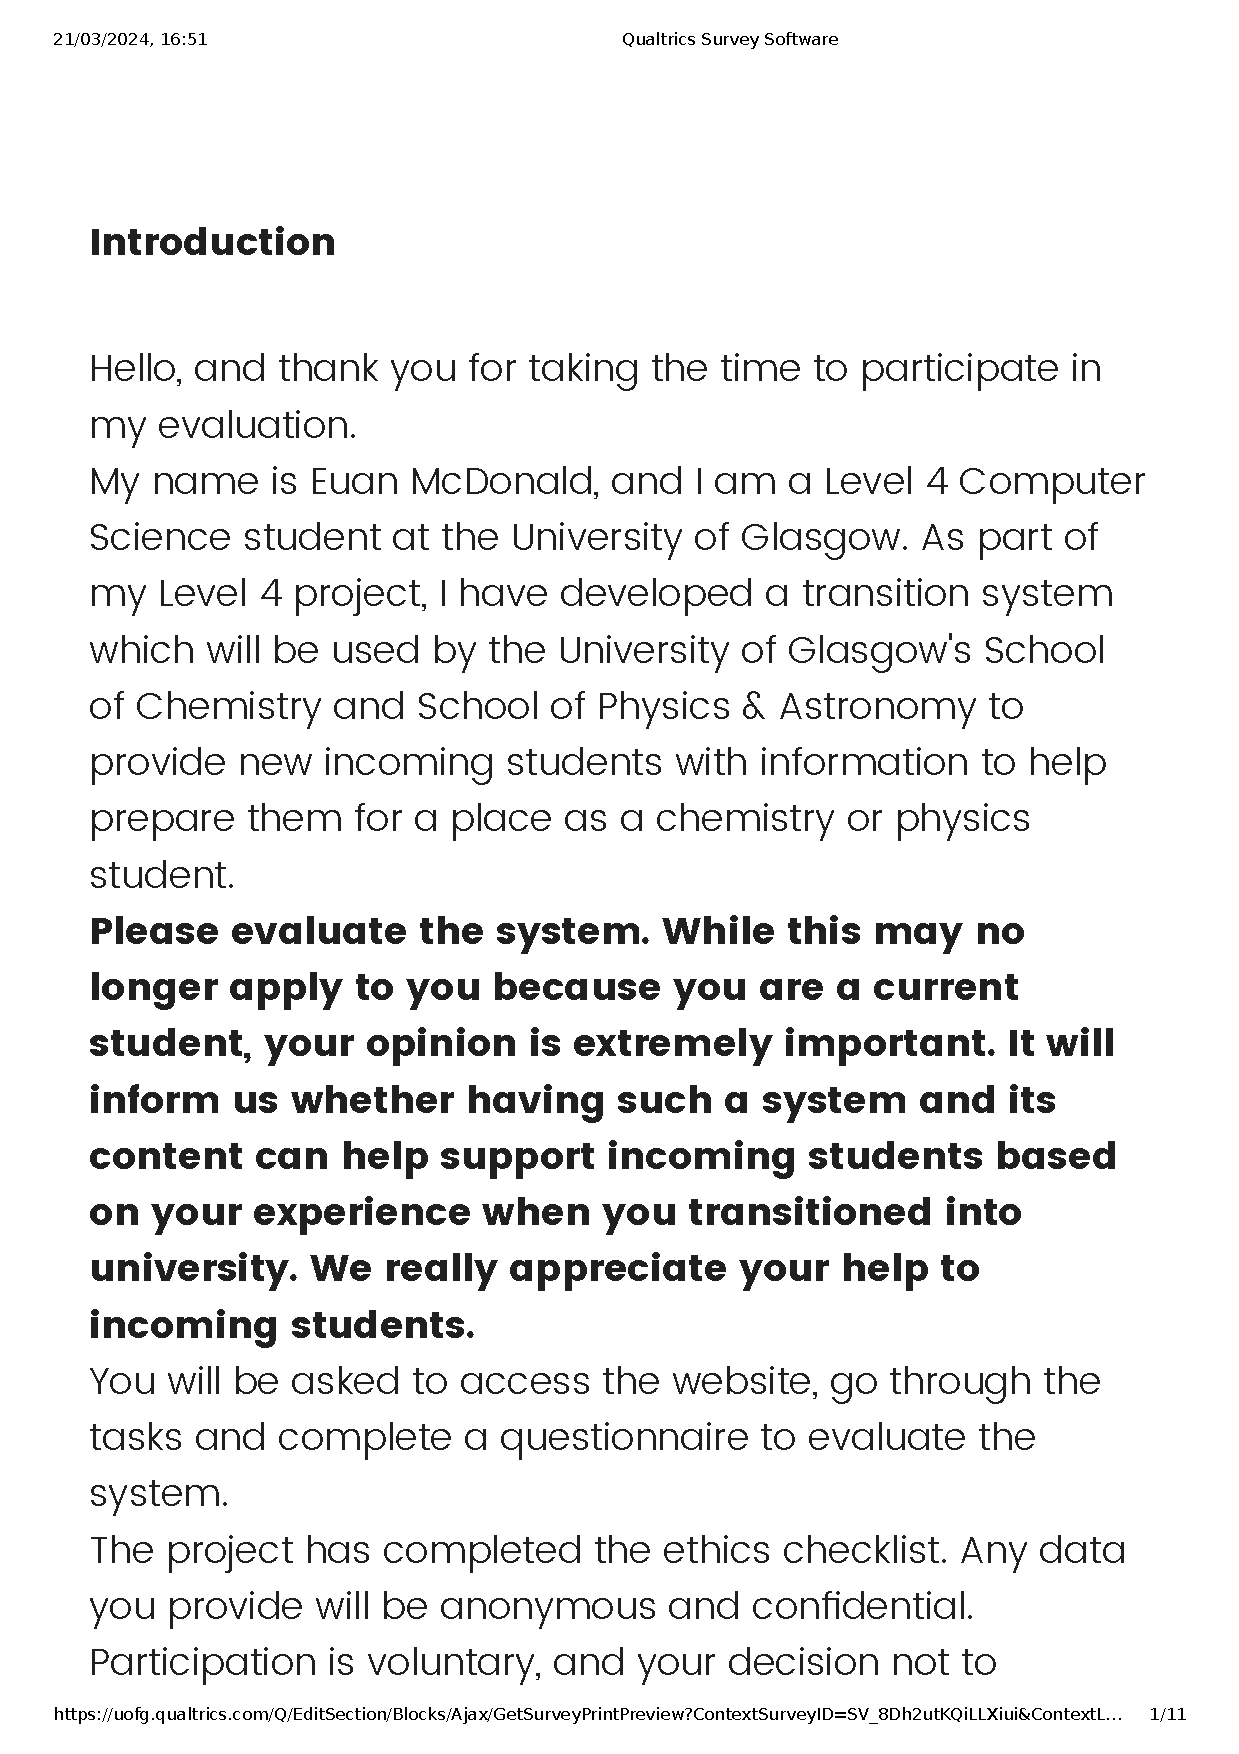
\includepdf[pages=-]{appendix/UniversityEvaluation.pdf}

\subsection{High School Student Evaluation} \label{app:evalHigh}
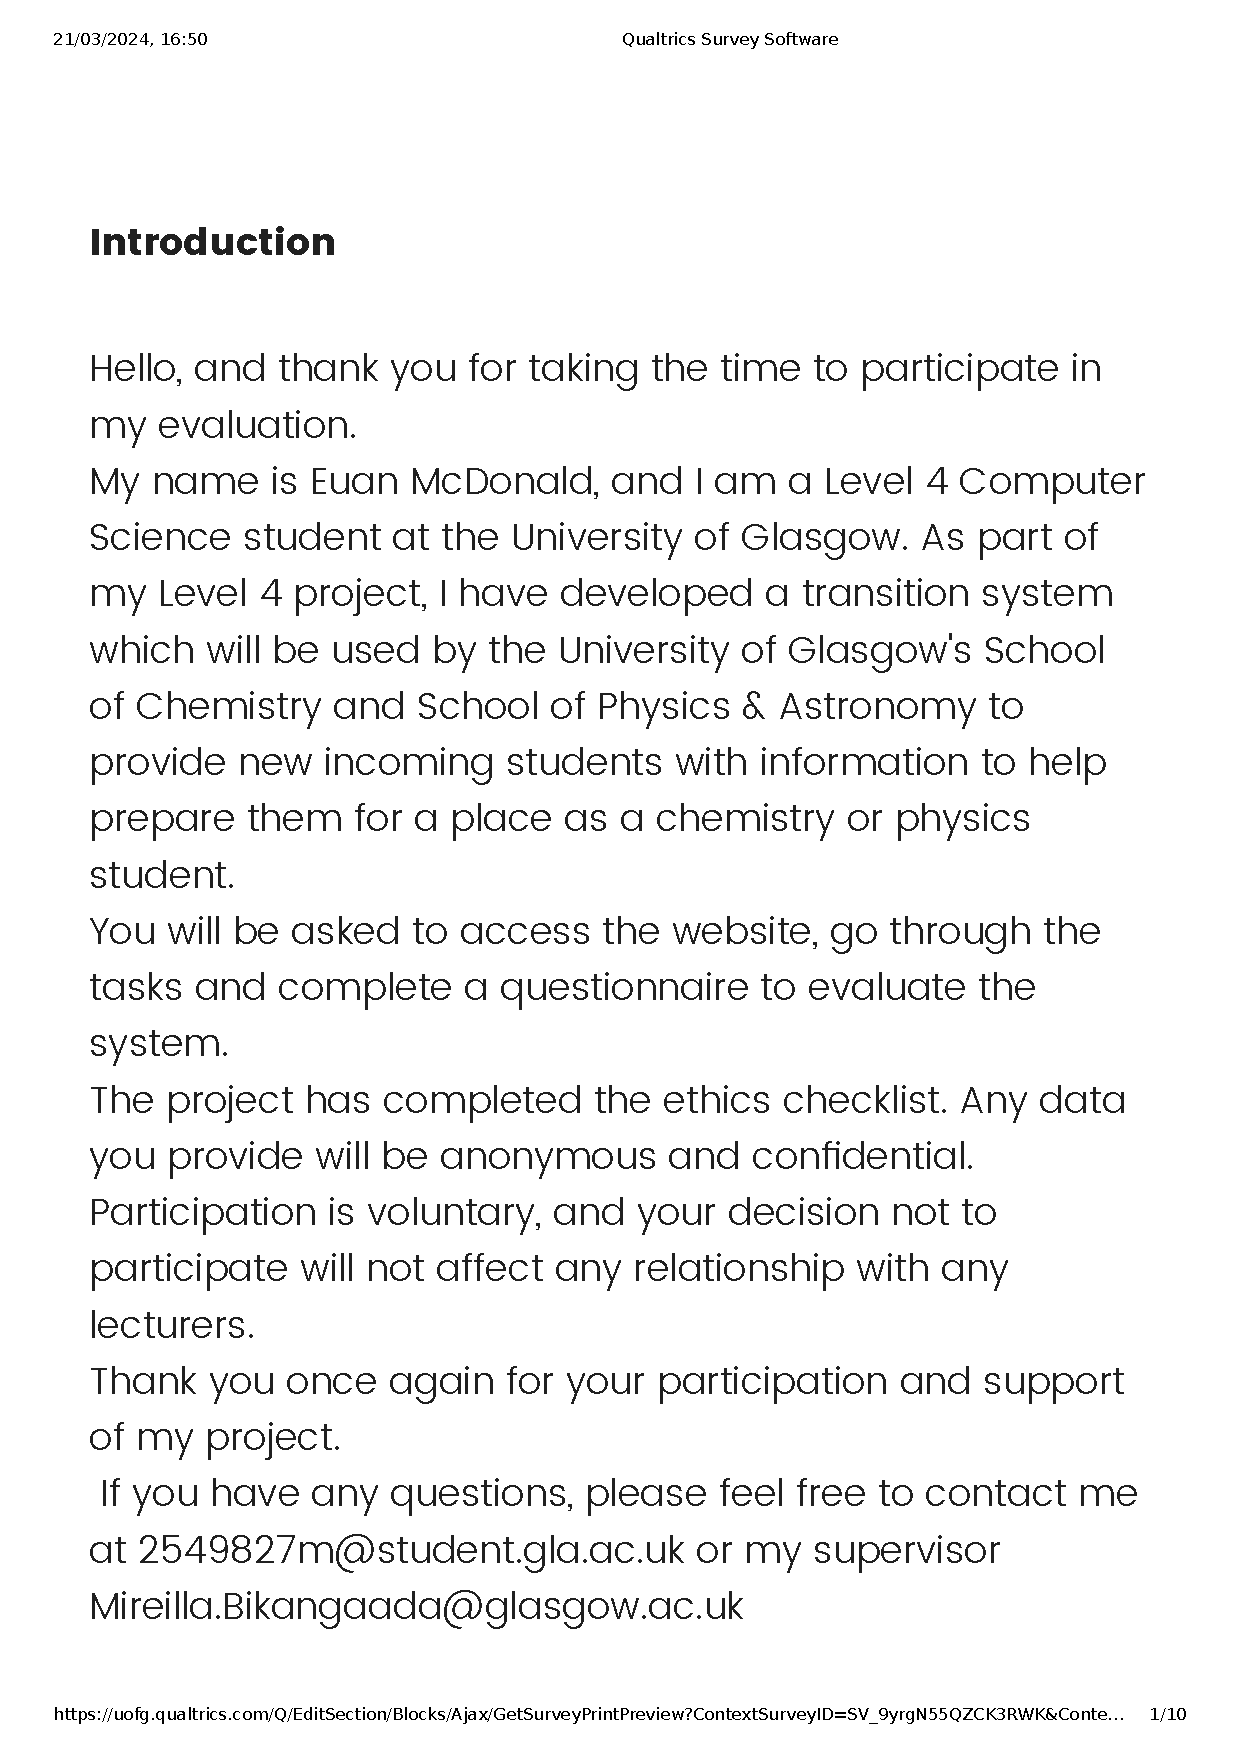
\includepdf[pages=-]{appendix/HighSchoolEvaluation.pdf}

\subsection{Transitions Working Group Evaluation} \label{app:evalTwg}
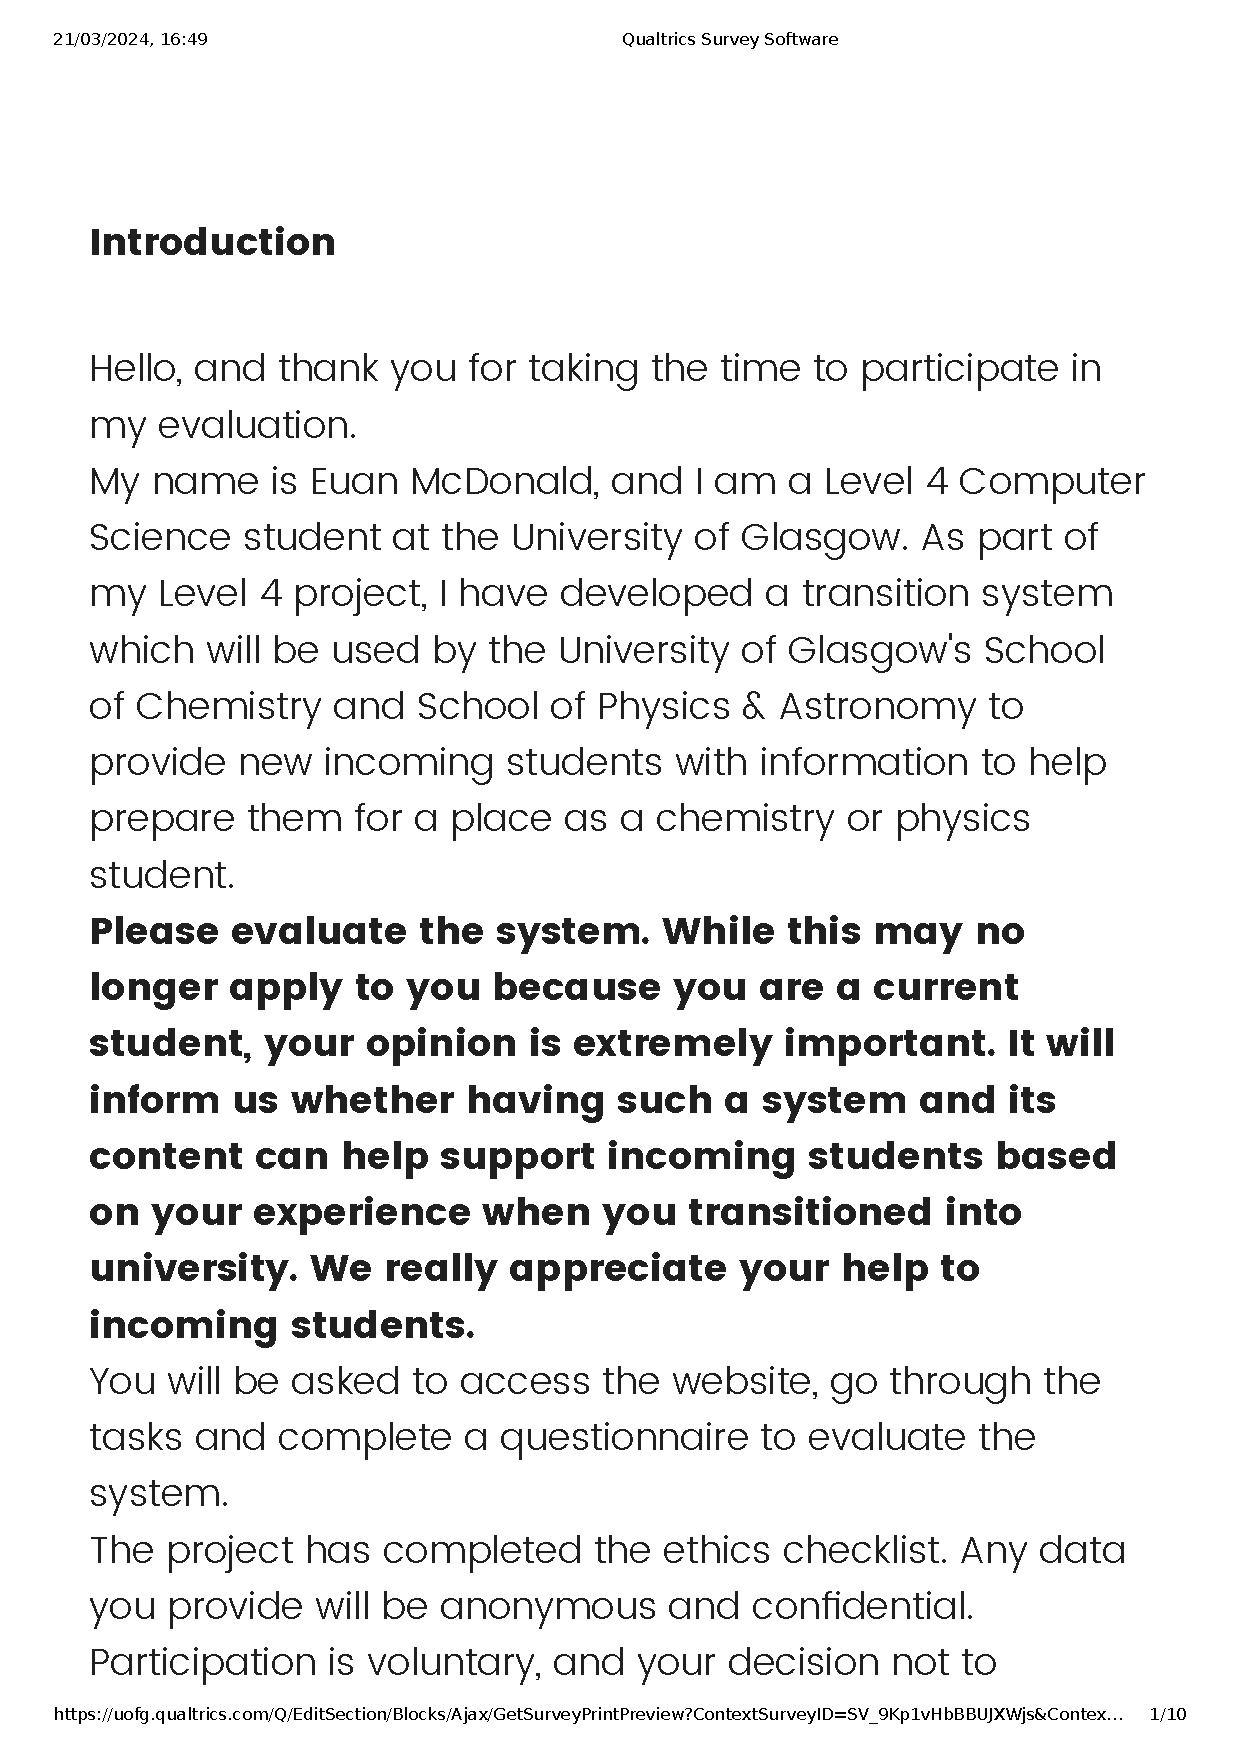
\includepdf[pages=-]{appendix/TWGEvaluation.pdf}

\section{}{Evaluation Results} \label{app:evalResults}
\subsection{University Student Evaluation Results} \label{app:evalUniResults}
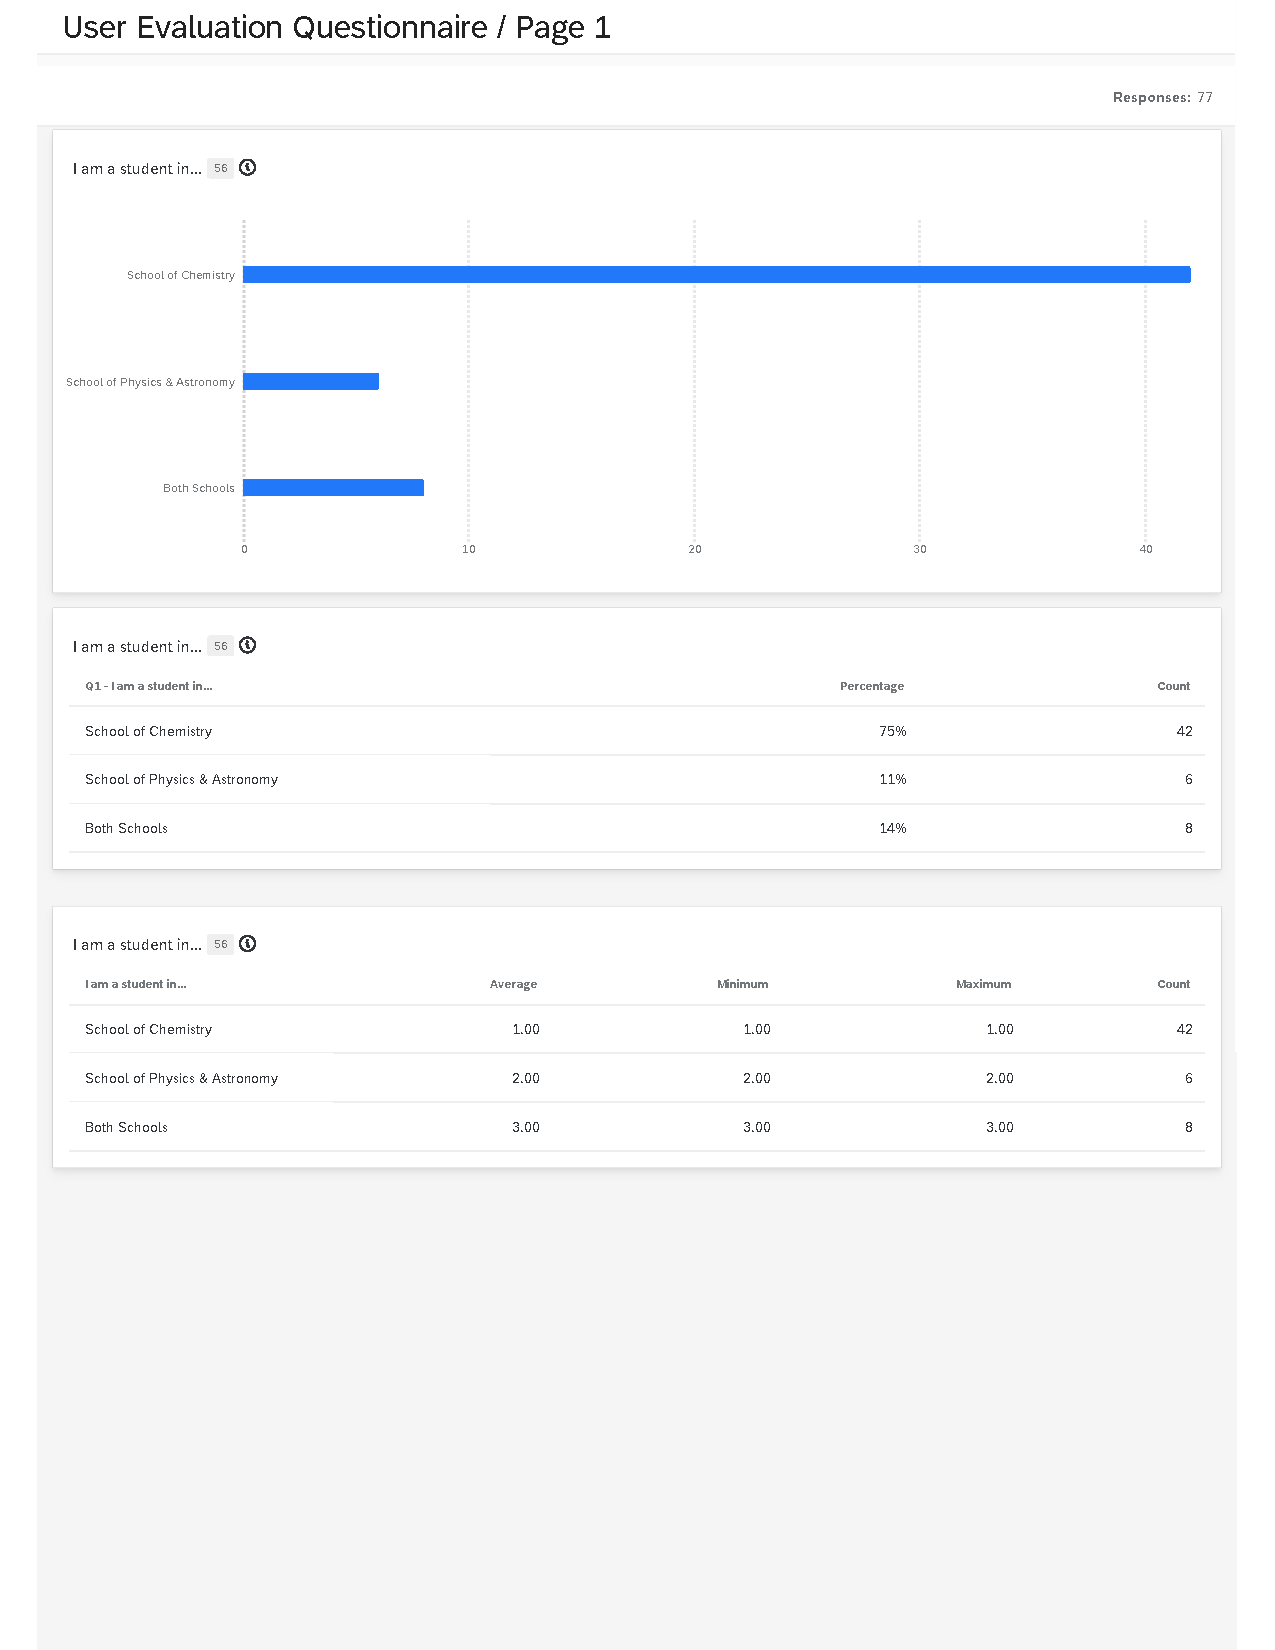
\includepdf[pages=-]{appendix/UniversityEvaluationResults.pdf}
 
\subsection{High School Student Evaluation Results} \label{app:evalHighResults}
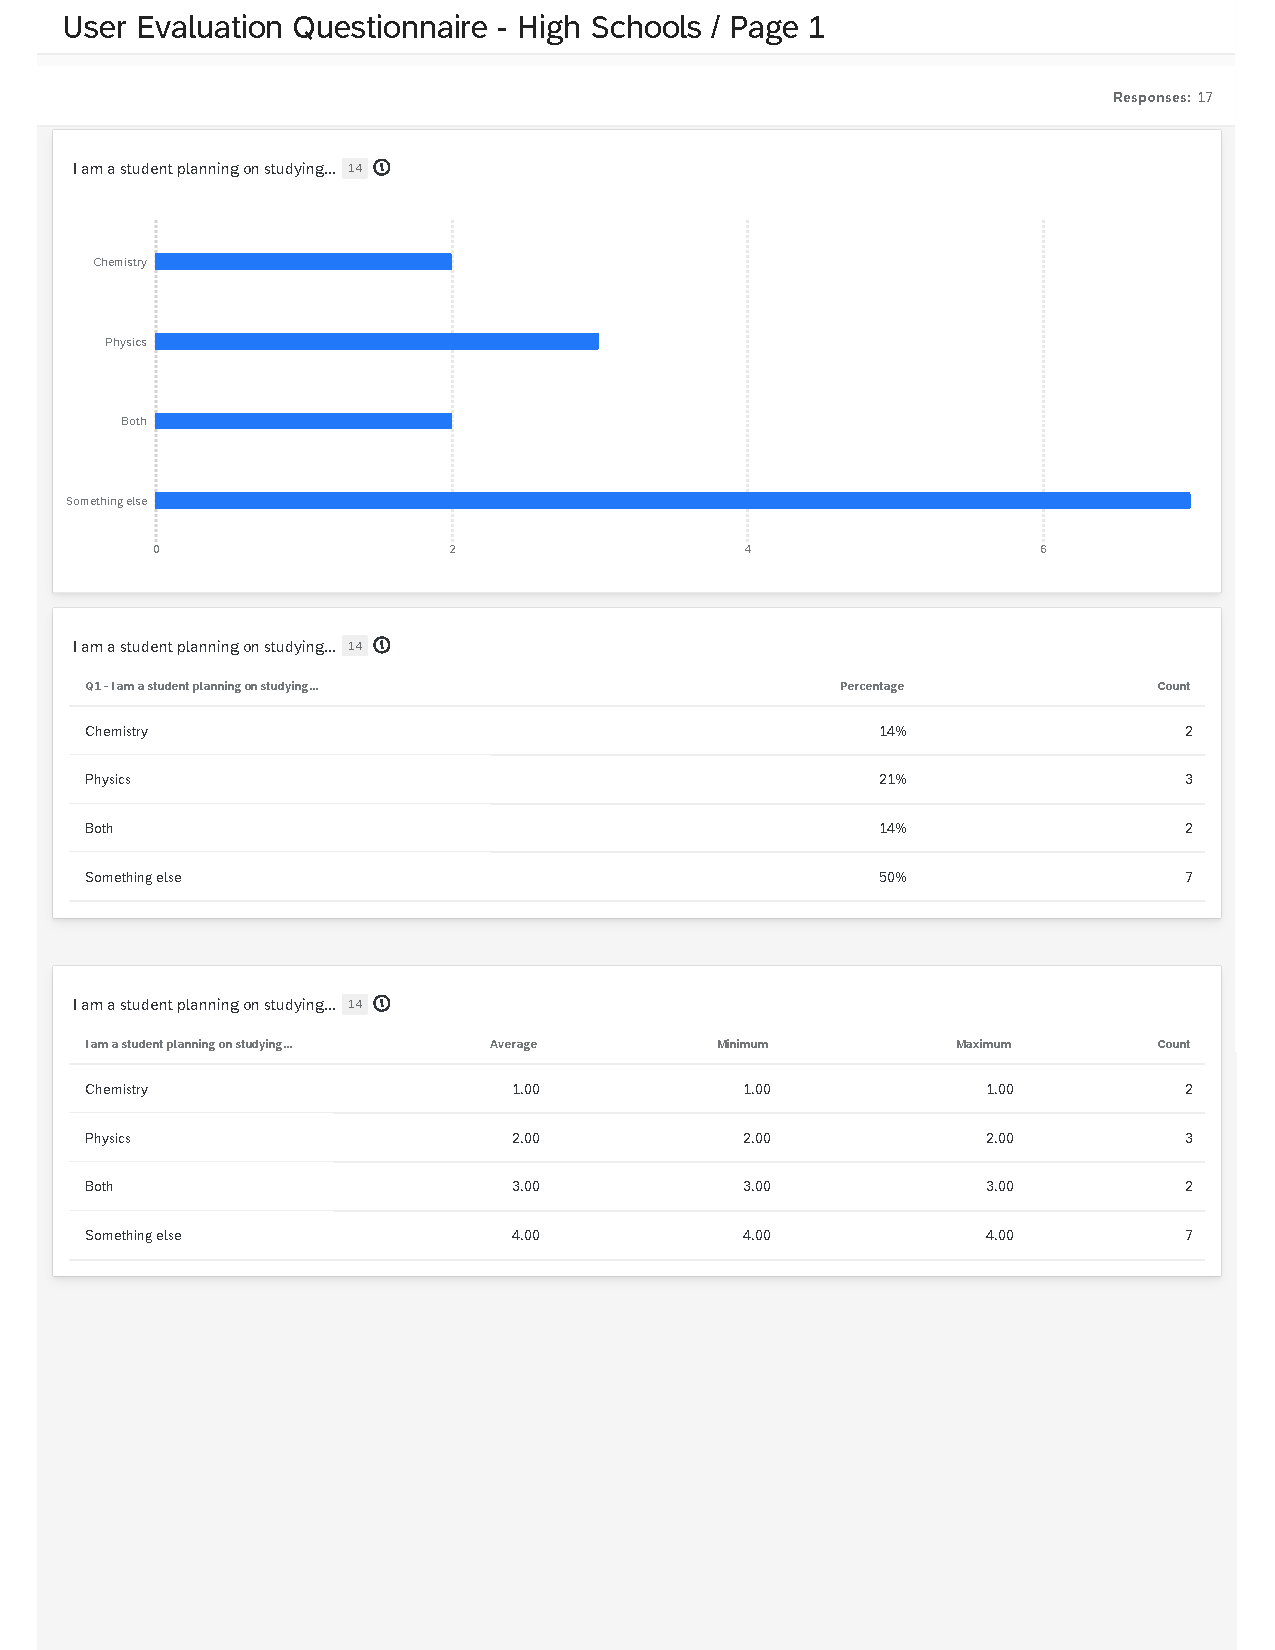
\includepdf[pages=-]{appendix/HighSchoolEvaluationResults.pdf}

\subsection{Transitions Working Group Evaluation Results} \label{app:evalTwgResults}
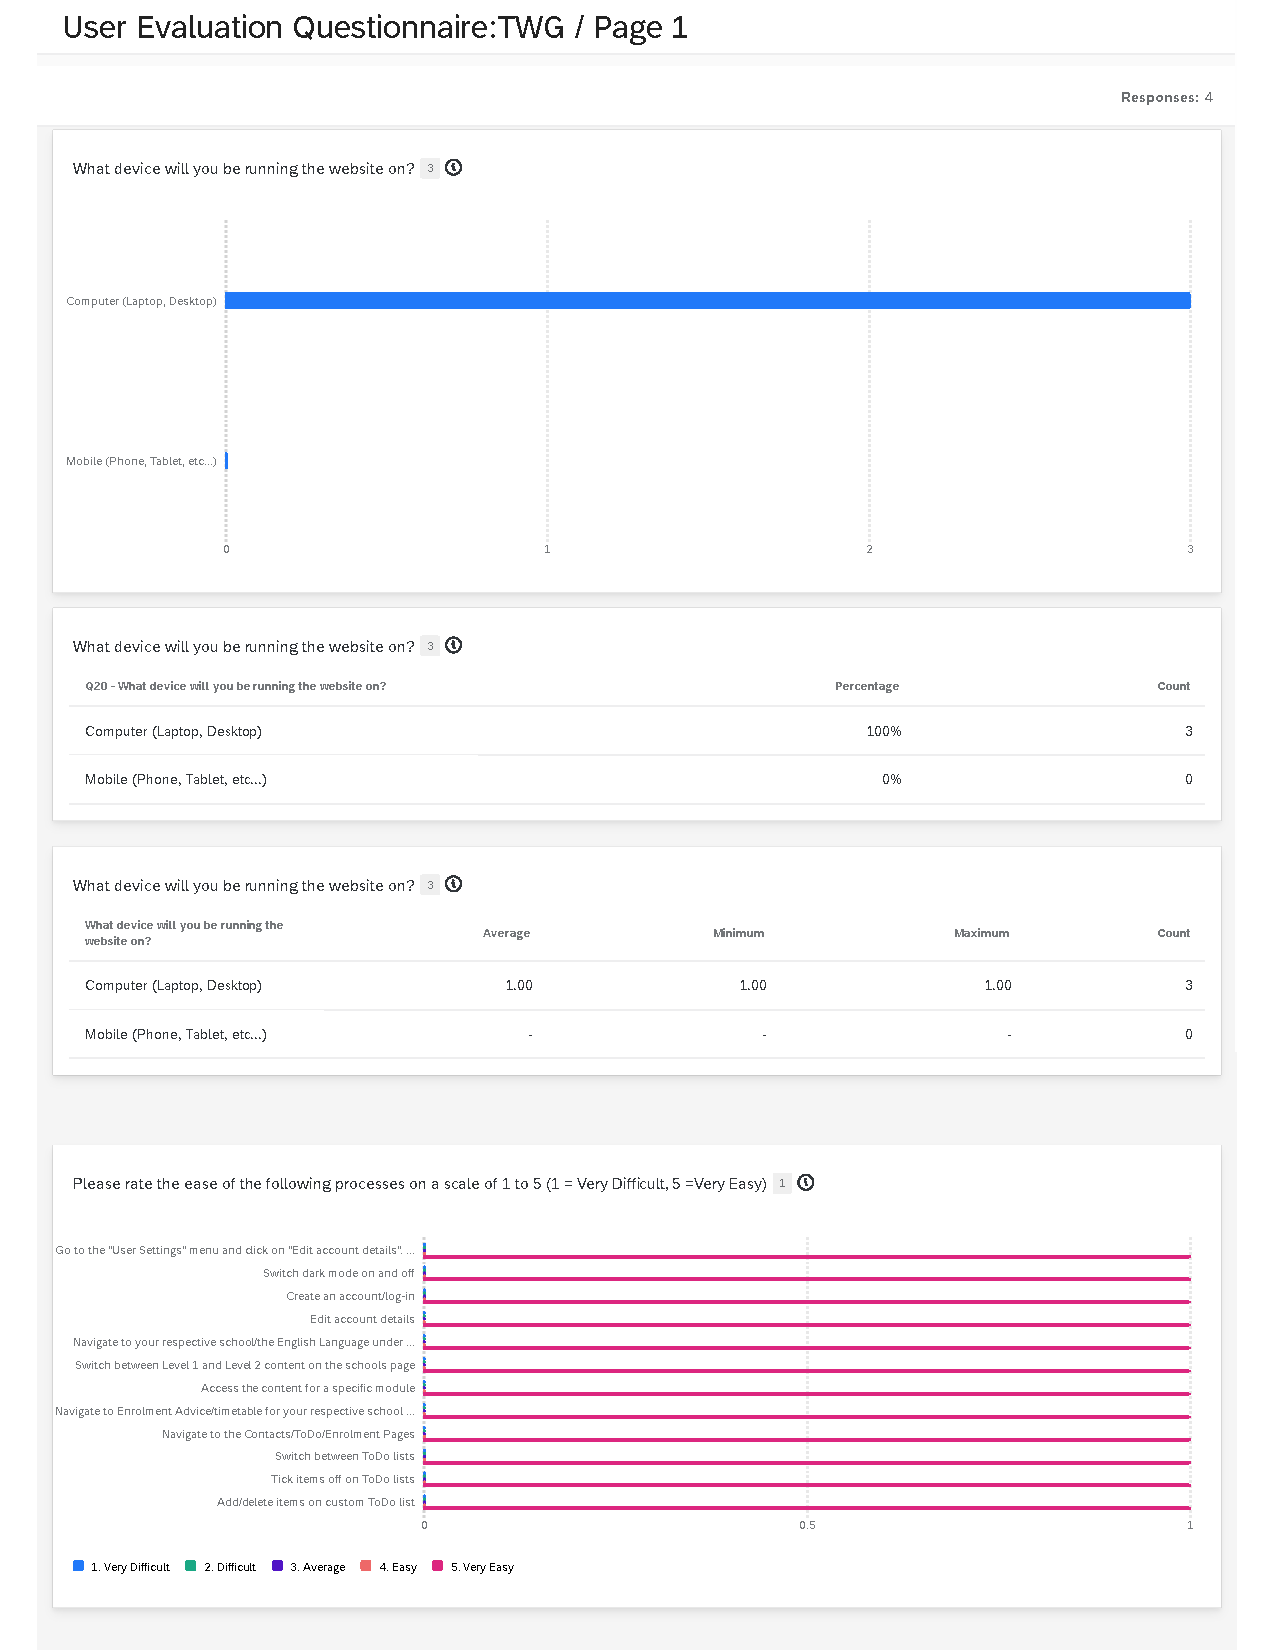
\includepdf[pages=-]{appendix/TWGEvaluationResults.pdf}

\chapter{State of Requirements} \label{app:reqMet}
\section{Functional Requirements} \label{app:funcMet}
\begin{table}[]
    \caption{Table showing the functional requirements of the application,  the MoSCoW categories Must Have and Should Have,  whether they are satisfied,  and reasoning for their status. }\label{tab:functionalApp}
    %\tt 
    \rowcolors{2}{}{gray!3}
    \begin{tabular}{ m{3cm}  m{2cm}  m{1.5cm}  m{17em} }
    %\toprule
    \hline
    \textbf{Requirement}    & \textbf{Category}                & \textbf{Satisfied}      & \textbf{Reason}                      \\ %\midrule % optional rule for header
    \hline
    
    Overview of Modules  &  Must Have              & Yes                 & The application provides a breakdown of each module covered in both Levels 1 \& 2 chemistry and physics as an overview and the aims. \\

    External English Language Resources & Must Have & Yes & The application contains a whole page dedicated to redirecting users to external language learning resources. \\

    Example Timetables & Must Have & Yes & The application provides an example of the chemistry and physics timetable fro both semester for Levels 1 \& 2. \\

    Pre-University To-Do List & Must Have & Yes & The application provides to-do lists telling users about tasks and items they should have completed before starting and that they should do in their first week. \\
    
    Links to Disability Service & Must Have & Yes & The contacts section of the application redirects users to the universities disabilities service page. \\
    
    Essential Contacts & Must Have & Yes & The application contains a section holding the key contacts that both schools wished to provide to incoming students. \\

    Enrolment and Module Selection Advice & Should Have & Partially & The application provides advice on module selection but not on enrolment. \\
    
    Personal To-Do List & Should Have & Yes & Users with an account have access to their own personalised to-do list which they can add and remove items from. \\
    
    Extracurricular Information & Should Have & Yes & The application links users to the universities student bodies as well as relevant clubs,  societies,  and groups. \\
    
    End-of-Unit Quizzes & Should Have & No & Due to difficulties in providing materials,  this feature was not included. \\
    
    Recommended Reading & Should Have & Partially & The physics modules have recommended readings,  however the chemistry modules do not. This is due to the materials provided by the schools. \\
    
    Additional Materials & Should Have & No & This is due to the materials not being provided by the schools. \\
    
    Edit Account Details & Should Have & Yes & Users can change the email and password associated with their account. \\

    % \bottomrule
    \end{tabular}
\end{table}

\section{Non-Functional Requirements} \label{app:nonFuncMet}

\begin{table}[]
    \caption{Table showing the functional requirements of the application,  the MoSCoW category Could Have,  whether they are satisfied,  and reasoning for their status. }\label{tab:functionalAppCont}
    %\tt 
    \rowcolors{2}{}{gray!3}
    \begin{tabular}{ m{3cm}  m{2cm}  m{1.5cm}  m{17em} }
    %\toprule
    \hline
    \textbf{Requirement}    & \textbf{Category}                & \textbf{Satisfied}      & \textbf{Reason}                      \\ %\midrule % optional rule for header
    \hline
         
    Mentor System & Could Have & No & This would have taken too long to gather resources and develop. \\
    
    Virtual Tour & Could Have & Yes & A link to an external resource including this is provided in the application. \\
    
    Testimonials & Could Have & No & Students did not reply when asked to give testimonials. \\
    
    Flashcards & Could Have & No & The application was to focus more on preparing students for starting university,  and not to be a general revision tool. \\
    
    High School Material Quizzes & Could Have & No & Quizzes were decided to focus on content covered in modules. \\
    
    Past Paper Questions & Could Have & No & Questions could not be provided by school for assessment reasons. \\
    
    Personal Calendar/Diary  & Could Have & No & The was not necessary to meet the applications aims. \\
    
    Programming Advice & Could Have & No & It was decided to focus more on the science aspects of Level 1 and 2 chemistry and physics. \\
    
    Forum System & Could Have & No & The contacts area meant that this was not needed as users could directly ask contacts any queries. \\
    
    Formula Sheets & Could Have & No & This would be provided when the content was taught in class and students had more of an understanding of equations.

    % \bottomrule
    \end{tabular}
\end{table}

\end{appendices}

%==================================================================================================================================
%   BIBLIOGRAPHY   

% The bibliography style is abbrvnat
% The bibliography always appears last,  after the appendices.

% to avoid "no citation" error
\nocite{*}

\bibliographystyle{abbrvnat}
\renewcommand{\thechapter}{0}
\bibliography{l4proj}

\end{document}
